% Cole Nielsen niels538@umn.edu
% EE 2002 Spring 2015
% Formal Lab Report 1

%----------------------------------------------------------------------------------------
%	PACKAGES AND DOCUMENT CONFIGURATIONS
%----------------------------------------------------------------------------------------

\documentclass[12pt]{article}

\usepackage{circuitikz}
\usepackage{graphicx}
\usepackage{subcaption}
\usepackage[top=1in, bottom= 1in, left=1in, right= 1in]{geometry}
\setlength\parindent{0pt}
\usepackage{fancyhdr}
\pagestyle{fancy}

%----------------------------------------------------------------------------------------
%	DOCUMENT INFORMATION
%----------------------------------------------------------------------------------------

\title{Experiment 4: I-V Curves  \\ and Load Lines \\ \vspace{0.3 in} EE 2002}

\author{Cole \textsc{Nielsen}} 
\date{Spring 2015}

\newcommand{\mymeter}[2]{   	% #1 = name , #2 = rotation angle
 \begin{scope}[transform shape,rotate=#2]
   \draw[thick] (#1)node(){$\mathbf V$} circle (11pt);
   \draw[rotate=45,-latex] (#1)  +(-17pt,0) --+(17pt,0);
 \end{scope}
}

\begin{document}
\maketitle 

\begin{center}
 \begin{tabular}{l r}
   Date Performed: & March 2, 2015 \\ 
   Instructor: & Rebecca Culp \\ 
\end{tabular}
\end{center}
\pagebreak

%----------------------------------------------------------------------------------------
%	Abstract
%----------------------------------------------------------------------------------------
\begin{abstract}
Load line and diode models were used to analyze and design several non-linear circuits. In particular, the I-V curve of an incandescent light bulb was found experimentally, showing a non-linear nature. Then using load lines, the current through the bulb was successfully predicted when connected to a resistor. The behavior of a diode connected a resistor and signal generator was also observed. In particular, it was determined that a diode conducts when a potential of 0.7 volts or more is present across the diode from anode to cathode (otherwise it behaves as an open circuit). It was also determined that the voltage dropped across a diode is generally 0.7 volts. Finally, several voltage clipper circuits were successfully designed to cut off a signal at different levels understanding the behavior of diodes. These results provide valuable insight into the design of non-linear and voltage clipping circuits.
\end{abstract}

%----------------------------------------------------------------------------------------
%	Introduction
%----------------------------------------------------------------------------------------
\section{Introduction}
%
I-V curves, load lines and diode models are powerful tools that are used to design circuits containing non-linear elements such as diodes and incandescent light bulbs. These models allow for effective control of parameters such as operating point and circuit response in non-linear circuits. I-V curves (current-voltage curves) are graphical representations used to show the relationship between the current running through a circuit element and the voltage across it. A typical I-V curve is that of a diode shown below. Diodes in the simplest sense are devices that only conduct current in one direction. They are constructed out of semiconductors- typically silicon- that are doped (have impurities added) in order to change the characteristics of the material. Diodes are built from two layers of semiconductors doped such that one layer has an excess of electrons relative to the other. This causes it so that currents will only flow through the diode in the direction that moves electrons from the layer with an excess of electrons to the other. \par 

\begin {figure}[htb!]
 \begin{center}
   \resizebox{0.6\textwidth}{!}{% GNUPLOT: LaTeX picture
\setlength{\unitlength}{0.240900pt}
\ifx\plotpoint\undefined\newsavebox{\plotpoint}\fi
\sbox{\plotpoint}{\rule[-0.200pt]{0.400pt}{0.400pt}}%
\begin{picture}(1500,900)(0,0)
\sbox{\plotpoint}{\rule[-0.200pt]{0.400pt}{0.400pt}}%
\put(211.0,131.0){\rule[-0.200pt]{4.818pt}{0.400pt}}
\put(191,131){\makebox(0,0)[r]{-0.005}}
\put(1419.0,131.0){\rule[-0.200pt]{4.818pt}{0.400pt}}
\put(211.0,260.0){\rule[-0.200pt]{4.818pt}{0.400pt}}
\put(191,260){\makebox(0,0)[r]{ 0}}
\put(1419.0,260.0){\rule[-0.200pt]{4.818pt}{0.400pt}}
\put(211.0,389.0){\rule[-0.200pt]{4.818pt}{0.400pt}}
\put(191,389){\makebox(0,0)[r]{ 0.005}}
\put(1419.0,389.0){\rule[-0.200pt]{4.818pt}{0.400pt}}
\put(211.0,518.0){\rule[-0.200pt]{4.818pt}{0.400pt}}
\put(191,518){\makebox(0,0)[r]{ 0.01}}
\put(1419.0,518.0){\rule[-0.200pt]{4.818pt}{0.400pt}}
\put(211.0,647.0){\rule[-0.200pt]{4.818pt}{0.400pt}}
\put(191,647){\makebox(0,0)[r]{ 0.015}}
\put(1419.0,647.0){\rule[-0.200pt]{4.818pt}{0.400pt}}
\put(211.0,776.0){\rule[-0.200pt]{4.818pt}{0.400pt}}
\put(191,776){\makebox(0,0)[r]{ 0.02}}
\put(1419.0,776.0){\rule[-0.200pt]{4.818pt}{0.400pt}}
\put(457.0,131.0){\rule[-0.200pt]{0.400pt}{4.818pt}}
\put(457,90){\makebox(0,0){ 0}}
\put(457.0,756.0){\rule[-0.200pt]{0.400pt}{4.818pt}}
\put(1144.0,131.0){\rule[-0.200pt]{0.400pt}{4.818pt}}
\put(1144,90){\makebox(0,0){ 0.7}}
\put(1144.0,756.0){\rule[-0.200pt]{0.400pt}{4.818pt}}
\put(211.0,131.0){\rule[-0.200pt]{0.400pt}{155.380pt}}
\put(211.0,131.0){\rule[-0.200pt]{295.825pt}{0.400pt}}
\put(1439.0,131.0){\rule[-0.200pt]{0.400pt}{155.380pt}}
\put(211.0,776.0){\rule[-0.200pt]{295.825pt}{0.400pt}}
\put(30,483){\makebox(0,0){\hspace{-0.5in}Current}}
\put(30,423){\makebox(0,0){\hspace{-0.5in}(A)}}
\put(825,29){\makebox(0,0){Voltage}}
\put(825,838){\makebox(0,0){\textbf{Figure 1.} Typical Diode I-V Curve}}
\put(211,260){\usebox{\plotpoint}}
\put(980,259.67){\rule{2.891pt}{0.400pt}}
\multiput(980.00,259.17)(6.000,1.000){2}{\rule{1.445pt}{0.400pt}}
\put(211.0,260.0){\rule[-0.200pt]{185.252pt}{0.400pt}}
\put(1005,260.67){\rule{2.891pt}{0.400pt}}
\multiput(1005.00,260.17)(6.000,1.000){2}{\rule{1.445pt}{0.400pt}}
\put(1017,261.67){\rule{3.132pt}{0.400pt}}
\multiput(1017.00,261.17)(6.500,1.000){2}{\rule{1.566pt}{0.400pt}}
\put(1030,263.17){\rule{2.500pt}{0.400pt}}
\multiput(1030.00,262.17)(6.811,2.000){2}{\rule{1.250pt}{0.400pt}}
\multiput(1042.00,265.61)(2.472,0.447){3}{\rule{1.700pt}{0.108pt}}
\multiput(1042.00,264.17)(8.472,3.000){2}{\rule{0.850pt}{0.400pt}}
\multiput(1054.00,268.60)(1.797,0.468){5}{\rule{1.400pt}{0.113pt}}
\multiput(1054.00,267.17)(10.094,4.000){2}{\rule{0.700pt}{0.400pt}}
\multiput(1067.00,272.59)(0.758,0.488){13}{\rule{0.700pt}{0.117pt}}
\multiput(1067.00,271.17)(10.547,8.000){2}{\rule{0.350pt}{0.400pt}}
\multiput(1079.00,280.58)(0.497,0.493){23}{\rule{0.500pt}{0.119pt}}
\multiput(1079.00,279.17)(11.962,13.000){2}{\rule{0.250pt}{0.400pt}}
\multiput(1092.58,293.00)(0.492,0.841){21}{\rule{0.119pt}{0.767pt}}
\multiput(1091.17,293.00)(12.000,18.409){2}{\rule{0.400pt}{0.383pt}}
\multiput(1104.58,313.00)(0.492,1.444){21}{\rule{0.119pt}{1.233pt}}
\multiput(1103.17,313.00)(12.000,31.440){2}{\rule{0.400pt}{0.617pt}}
\multiput(1116.58,347.00)(0.493,2.122){23}{\rule{0.119pt}{1.762pt}}
\multiput(1115.17,347.00)(13.000,50.344){2}{\rule{0.400pt}{0.881pt}}
\multiput(1129.58,401.00)(0.492,3.813){21}{\rule{0.119pt}{3.067pt}}
\multiput(1128.17,401.00)(12.000,82.635){2}{\rule{0.400pt}{1.533pt}}
\multiput(1141.58,490.00)(0.493,5.651){23}{\rule{0.119pt}{4.500pt}}
\multiput(1140.17,490.00)(13.000,133.660){2}{\rule{0.400pt}{2.250pt}}
\multiput(1154.59,633.00)(0.485,10.866){11}{\rule{0.117pt}{8.271pt}}
\multiput(1153.17,633.00)(7.000,125.832){2}{\rule{0.400pt}{4.136pt}}
\put(992.0,261.0){\rule[-0.200pt]{3.132pt}{0.400pt}}
\put(211.0,131.0){\rule[-0.200pt]{0.400pt}{155.380pt}}
\put(211.0,131.0){\rule[-0.200pt]{295.825pt}{0.400pt}}
\put(1439.0,131.0){\rule[-0.200pt]{0.400pt}{155.380pt}}
\put(211.0,776.0){\rule[-0.200pt]{295.825pt}{0.400pt}}
\end{picture}
}
 \end{center}
\end {figure}

As seen above in the diode I-V curve, a diode conducts essentially zero current (is an open circuit) until it reaches a threshold voltage where the diode begins to conduct as if it is a short. For most diodes like the one in \textit{Figure 1}, this voltage is approximately 0.7 V. The voltage drop with respect to current grows very slowly after 0.7 volts, remaining almost constant. Because of this, the voltage dropped across a conducting diode is usually generalized as 0.7 V. Using a fixed voltage drop model for diodes in circuit analysis greatly simplifies the process by removing the need to use complex exponential functions like the Shockley diode equation. \\\par
%
In this experiment an incandescent light bulb's I-V curve was determined. An incandescent light bulb is simply a resistor that is designed to heat up and emit light as current flows through it. Its I-V curve is of particular interest due to its non-linear nature which is unexpected from a resistor. Usually resistor I-V curves are linear, being determined by ohms law (\(V = IR\)). The IV curve of a light bulb changes much more gradually than than that of a diode, making it a good example for load line analysis to determine the operating point of a non-linear circuit. A load line is a graphical method using I-V curves to determine the operating state of a circuit with non-linear elements. The I-V curves of two elements being considered are graphed on the same plot and the intersection of the the curves represents what is called the operating point. The operating point is what voltage and current the circuit will operate at.  Below is an example load line for a Th\'{e}venin equivalent voltage source connected to a diode. The diode's I-V curve is modelled by the Shockley Diode equation, also shown below.\par
%
\begin {figure}[htb!]
 \begin{center}
   \resizebox{0.6\textwidth}{!}{% GNUPLOT: LaTeX picture
\setlength{\unitlength}{0.240900pt}
\ifx\plotpoint\undefined\newsavebox{\plotpoint}\fi
\begin{picture}(1500,900)(0,0)
\sbox{\plotpoint}{\rule[-0.200pt]{0.400pt}{0.400pt}}%
\put(71.0,69.0){\rule[-0.200pt]{0.400pt}{170.316pt}}
\put(71.0,69.0){\rule[-0.200pt]{329.551pt}{0.400pt}}
\put(1439.0,69.0){\rule[-0.200pt]{0.400pt}{170.316pt}}
\put(71.0,776.0){\rule[-0.200pt]{329.551pt}{0.400pt}}
\put(30,422){\makebox(0,0){\hspace{-0.5in}Current}}
\put(755,29){\makebox(0,0){Voltage}}
\put(755,838){\makebox(0,0){\textbf{Figure 2.} Line Example}}
\put(71,103){\usebox{\plotpoint}}
\put(803,102.67){\rule{3.373pt}{0.400pt}}
\multiput(803.00,102.17)(7.000,1.000){2}{\rule{1.686pt}{0.400pt}}
\put(71.0,103.0){\rule[-0.200pt]{176.339pt}{0.400pt}}
\put(831,103.67){\rule{3.373pt}{0.400pt}}
\multiput(831.00,103.17)(7.000,1.000){2}{\rule{1.686pt}{0.400pt}}
\put(817.0,104.0){\rule[-0.200pt]{3.373pt}{0.400pt}}
\put(859,105.17){\rule{2.700pt}{0.400pt}}
\multiput(859.00,104.17)(7.396,2.000){2}{\rule{1.350pt}{0.400pt}}
\put(872,107.17){\rule{2.900pt}{0.400pt}}
\multiput(872.00,106.17)(7.981,2.000){2}{\rule{1.450pt}{0.400pt}}
\multiput(886.00,109.61)(2.918,0.447){3}{\rule{1.967pt}{0.108pt}}
\multiput(886.00,108.17)(9.918,3.000){2}{\rule{0.983pt}{0.400pt}}
\multiput(900.00,112.60)(1.943,0.468){5}{\rule{1.500pt}{0.113pt}}
\multiput(900.00,111.17)(10.887,4.000){2}{\rule{0.750pt}{0.400pt}}
\multiput(914.00,116.59)(1.214,0.482){9}{\rule{1.033pt}{0.116pt}}
\multiput(914.00,115.17)(11.855,6.000){2}{\rule{0.517pt}{0.400pt}}
\multiput(928.00,122.58)(0.704,0.491){17}{\rule{0.660pt}{0.118pt}}
\multiput(928.00,121.17)(12.630,10.000){2}{\rule{0.330pt}{0.400pt}}
\multiput(942.58,132.00)(0.493,0.536){23}{\rule{0.119pt}{0.531pt}}
\multiput(941.17,132.00)(13.000,12.898){2}{\rule{0.400pt}{0.265pt}}
\multiput(955.58,146.00)(0.494,0.717){25}{\rule{0.119pt}{0.671pt}}
\multiput(954.17,146.00)(14.000,18.606){2}{\rule{0.400pt}{0.336pt}}
\multiput(969.58,166.00)(0.494,1.084){25}{\rule{0.119pt}{0.957pt}}
\multiput(968.17,166.00)(14.000,28.013){2}{\rule{0.400pt}{0.479pt}}
\multiput(983.58,196.00)(0.494,1.599){25}{\rule{0.119pt}{1.357pt}}
\multiput(982.17,196.00)(14.000,41.183){2}{\rule{0.400pt}{0.679pt}}
\multiput(997.58,240.00)(0.494,2.407){25}{\rule{0.119pt}{1.986pt}}
\multiput(996.17,240.00)(14.000,61.879){2}{\rule{0.400pt}{0.993pt}}
\multiput(1011.58,306.00)(0.493,3.787){23}{\rule{0.119pt}{3.054pt}}
\multiput(1010.17,306.00)(13.000,89.662){2}{\rule{0.400pt}{1.527pt}}
\multiput(1024.58,402.00)(0.494,5.234){25}{\rule{0.119pt}{4.186pt}}
\multiput(1023.17,402.00)(14.000,134.312){2}{\rule{0.400pt}{2.093pt}}
\multiput(1038.58,545.00)(0.494,7.658){25}{\rule{0.119pt}{6.071pt}}
\multiput(1037.17,545.00)(14.000,196.398){2}{\rule{0.400pt}{3.036pt}}
\put(1051.67,754){\rule{0.400pt}{5.300pt}}
\multiput(1051.17,754.00)(1.000,11.000){2}{\rule{0.400pt}{2.650pt}}
\put(845.0,105.0){\rule[-0.200pt]{3.373pt}{0.400pt}}
\put(71,776){\usebox{\plotpoint}}
\multiput(71.00,774.93)(0.890,-0.488){13}{\rule{0.800pt}{0.117pt}}
\multiput(71.00,775.17)(12.340,-8.000){2}{\rule{0.400pt}{0.400pt}}
\multiput(85.00,766.93)(1.026,-0.485){11}{\rule{0.900pt}{0.117pt}}
\multiput(85.00,767.17)(12.132,-7.000){2}{\rule{0.450pt}{0.400pt}}
\multiput(99.00,759.93)(0.824,-0.488){13}{\rule{0.750pt}{0.117pt}}
\multiput(99.00,760.17)(11.443,-8.000){2}{\rule{0.375pt}{0.400pt}}
\multiput(112.00,751.93)(0.890,-0.488){13}{\rule{0.800pt}{0.117pt}}
\multiput(112.00,752.17)(12.340,-8.000){2}{\rule{0.400pt}{0.400pt}}
\multiput(126.00,743.93)(1.026,-0.485){11}{\rule{0.900pt}{0.117pt}}
\multiput(126.00,744.17)(12.132,-7.000){2}{\rule{0.450pt}{0.400pt}}
\multiput(140.00,736.93)(0.890,-0.488){13}{\rule{0.800pt}{0.117pt}}
\multiput(140.00,737.17)(12.340,-8.000){2}{\rule{0.400pt}{0.400pt}}
\multiput(154.00,728.93)(0.890,-0.488){13}{\rule{0.800pt}{0.117pt}}
\multiput(154.00,729.17)(12.340,-8.000){2}{\rule{0.400pt}{0.400pt}}
\multiput(168.00,720.93)(1.026,-0.485){11}{\rule{0.900pt}{0.117pt}}
\multiput(168.00,721.17)(12.132,-7.000){2}{\rule{0.450pt}{0.400pt}}
\multiput(182.00,713.93)(0.824,-0.488){13}{\rule{0.750pt}{0.117pt}}
\multiput(182.00,714.17)(11.443,-8.000){2}{\rule{0.375pt}{0.400pt}}
\multiput(195.00,705.93)(0.890,-0.488){13}{\rule{0.800pt}{0.117pt}}
\multiput(195.00,706.17)(12.340,-8.000){2}{\rule{0.400pt}{0.400pt}}
\multiput(209.00,697.93)(0.890,-0.488){13}{\rule{0.800pt}{0.117pt}}
\multiput(209.00,698.17)(12.340,-8.000){2}{\rule{0.400pt}{0.400pt}}
\multiput(223.00,689.93)(1.026,-0.485){11}{\rule{0.900pt}{0.117pt}}
\multiput(223.00,690.17)(12.132,-7.000){2}{\rule{0.450pt}{0.400pt}}
\multiput(237.00,682.93)(0.890,-0.488){13}{\rule{0.800pt}{0.117pt}}
\multiput(237.00,683.17)(12.340,-8.000){2}{\rule{0.400pt}{0.400pt}}
\multiput(251.00,674.93)(0.824,-0.488){13}{\rule{0.750pt}{0.117pt}}
\multiput(251.00,675.17)(11.443,-8.000){2}{\rule{0.375pt}{0.400pt}}
\multiput(264.00,666.93)(1.026,-0.485){11}{\rule{0.900pt}{0.117pt}}
\multiput(264.00,667.17)(12.132,-7.000){2}{\rule{0.450pt}{0.400pt}}
\multiput(278.00,659.93)(0.890,-0.488){13}{\rule{0.800pt}{0.117pt}}
\multiput(278.00,660.17)(12.340,-8.000){2}{\rule{0.400pt}{0.400pt}}
\multiput(292.00,651.93)(0.890,-0.488){13}{\rule{0.800pt}{0.117pt}}
\multiput(292.00,652.17)(12.340,-8.000){2}{\rule{0.400pt}{0.400pt}}
\multiput(306.00,643.93)(1.026,-0.485){11}{\rule{0.900pt}{0.117pt}}
\multiput(306.00,644.17)(12.132,-7.000){2}{\rule{0.450pt}{0.400pt}}
\multiput(320.00,636.93)(0.890,-0.488){13}{\rule{0.800pt}{0.117pt}}
\multiput(320.00,637.17)(12.340,-8.000){2}{\rule{0.400pt}{0.400pt}}
\multiput(334.00,628.93)(0.824,-0.488){13}{\rule{0.750pt}{0.117pt}}
\multiput(334.00,629.17)(11.443,-8.000){2}{\rule{0.375pt}{0.400pt}}
\multiput(347.00,620.93)(1.026,-0.485){11}{\rule{0.900pt}{0.117pt}}
\multiput(347.00,621.17)(12.132,-7.000){2}{\rule{0.450pt}{0.400pt}}
\multiput(361.00,613.93)(0.890,-0.488){13}{\rule{0.800pt}{0.117pt}}
\multiput(361.00,614.17)(12.340,-8.000){2}{\rule{0.400pt}{0.400pt}}
\multiput(375.00,605.93)(0.890,-0.488){13}{\rule{0.800pt}{0.117pt}}
\multiput(375.00,606.17)(12.340,-8.000){2}{\rule{0.400pt}{0.400pt}}
\multiput(389.00,597.93)(1.026,-0.485){11}{\rule{0.900pt}{0.117pt}}
\multiput(389.00,598.17)(12.132,-7.000){2}{\rule{0.450pt}{0.400pt}}
\multiput(403.00,590.93)(0.824,-0.488){13}{\rule{0.750pt}{0.117pt}}
\multiput(403.00,591.17)(11.443,-8.000){2}{\rule{0.375pt}{0.400pt}}
\multiput(416.00,582.93)(0.890,-0.488){13}{\rule{0.800pt}{0.117pt}}
\multiput(416.00,583.17)(12.340,-8.000){2}{\rule{0.400pt}{0.400pt}}
\multiput(430.00,574.93)(0.890,-0.488){13}{\rule{0.800pt}{0.117pt}}
\multiput(430.00,575.17)(12.340,-8.000){2}{\rule{0.400pt}{0.400pt}}
\multiput(444.00,566.93)(1.026,-0.485){11}{\rule{0.900pt}{0.117pt}}
\multiput(444.00,567.17)(12.132,-7.000){2}{\rule{0.450pt}{0.400pt}}
\multiput(458.00,559.93)(0.890,-0.488){13}{\rule{0.800pt}{0.117pt}}
\multiput(458.00,560.17)(12.340,-8.000){2}{\rule{0.400pt}{0.400pt}}
\multiput(472.00,551.93)(0.890,-0.488){13}{\rule{0.800pt}{0.117pt}}
\multiput(472.00,552.17)(12.340,-8.000){2}{\rule{0.400pt}{0.400pt}}
\multiput(486.00,543.93)(0.950,-0.485){11}{\rule{0.843pt}{0.117pt}}
\multiput(486.00,544.17)(11.251,-7.000){2}{\rule{0.421pt}{0.400pt}}
\multiput(499.00,536.93)(0.890,-0.488){13}{\rule{0.800pt}{0.117pt}}
\multiput(499.00,537.17)(12.340,-8.000){2}{\rule{0.400pt}{0.400pt}}
\multiput(513.00,528.93)(0.890,-0.488){13}{\rule{0.800pt}{0.117pt}}
\multiput(513.00,529.17)(12.340,-8.000){2}{\rule{0.400pt}{0.400pt}}
\multiput(527.00,520.93)(1.026,-0.485){11}{\rule{0.900pt}{0.117pt}}
\multiput(527.00,521.17)(12.132,-7.000){2}{\rule{0.450pt}{0.400pt}}
\multiput(541.00,513.93)(0.890,-0.488){13}{\rule{0.800pt}{0.117pt}}
\multiput(541.00,514.17)(12.340,-8.000){2}{\rule{0.400pt}{0.400pt}}
\multiput(555.00,505.93)(0.824,-0.488){13}{\rule{0.750pt}{0.117pt}}
\multiput(555.00,506.17)(11.443,-8.000){2}{\rule{0.375pt}{0.400pt}}
\multiput(568.00,497.93)(1.026,-0.485){11}{\rule{0.900pt}{0.117pt}}
\multiput(568.00,498.17)(12.132,-7.000){2}{\rule{0.450pt}{0.400pt}}
\multiput(582.00,490.93)(0.890,-0.488){13}{\rule{0.800pt}{0.117pt}}
\multiput(582.00,491.17)(12.340,-8.000){2}{\rule{0.400pt}{0.400pt}}
\multiput(596.00,482.93)(0.890,-0.488){13}{\rule{0.800pt}{0.117pt}}
\multiput(596.00,483.17)(12.340,-8.000){2}{\rule{0.400pt}{0.400pt}}
\multiput(610.00,474.93)(1.026,-0.485){11}{\rule{0.900pt}{0.117pt}}
\multiput(610.00,475.17)(12.132,-7.000){2}{\rule{0.450pt}{0.400pt}}
\multiput(624.00,467.93)(0.890,-0.488){13}{\rule{0.800pt}{0.117pt}}
\multiput(624.00,468.17)(12.340,-8.000){2}{\rule{0.400pt}{0.400pt}}
\multiput(638.00,459.93)(0.824,-0.488){13}{\rule{0.750pt}{0.117pt}}
\multiput(638.00,460.17)(11.443,-8.000){2}{\rule{0.375pt}{0.400pt}}
\multiput(651.00,451.93)(1.026,-0.485){11}{\rule{0.900pt}{0.117pt}}
\multiput(651.00,452.17)(12.132,-7.000){2}{\rule{0.450pt}{0.400pt}}
\multiput(665.00,444.93)(0.890,-0.488){13}{\rule{0.800pt}{0.117pt}}
\multiput(665.00,445.17)(12.340,-8.000){2}{\rule{0.400pt}{0.400pt}}
\multiput(679.00,436.93)(0.890,-0.488){13}{\rule{0.800pt}{0.117pt}}
\multiput(679.00,437.17)(12.340,-8.000){2}{\rule{0.400pt}{0.400pt}}
\multiput(693.00,428.93)(0.890,-0.488){13}{\rule{0.800pt}{0.117pt}}
\multiput(693.00,429.17)(12.340,-8.000){2}{\rule{0.400pt}{0.400pt}}
\multiput(707.00,420.93)(0.950,-0.485){11}{\rule{0.843pt}{0.117pt}}
\multiput(707.00,421.17)(11.251,-7.000){2}{\rule{0.421pt}{0.400pt}}
\multiput(720.00,413.93)(0.890,-0.488){13}{\rule{0.800pt}{0.117pt}}
\multiput(720.00,414.17)(12.340,-8.000){2}{\rule{0.400pt}{0.400pt}}
\multiput(734.00,405.93)(0.890,-0.488){13}{\rule{0.800pt}{0.117pt}}
\multiput(734.00,406.17)(12.340,-8.000){2}{\rule{0.400pt}{0.400pt}}
\multiput(748.00,397.93)(1.026,-0.485){11}{\rule{0.900pt}{0.117pt}}
\multiput(748.00,398.17)(12.132,-7.000){2}{\rule{0.450pt}{0.400pt}}
\multiput(762.00,390.93)(0.890,-0.488){13}{\rule{0.800pt}{0.117pt}}
\multiput(762.00,391.17)(12.340,-8.000){2}{\rule{0.400pt}{0.400pt}}
\multiput(776.00,382.93)(0.890,-0.488){13}{\rule{0.800pt}{0.117pt}}
\multiput(776.00,383.17)(12.340,-8.000){2}{\rule{0.400pt}{0.400pt}}
\multiput(790.00,374.93)(0.950,-0.485){11}{\rule{0.843pt}{0.117pt}}
\multiput(790.00,375.17)(11.251,-7.000){2}{\rule{0.421pt}{0.400pt}}
\multiput(803.00,367.93)(0.890,-0.488){13}{\rule{0.800pt}{0.117pt}}
\multiput(803.00,368.17)(12.340,-8.000){2}{\rule{0.400pt}{0.400pt}}
\multiput(817.00,359.93)(0.890,-0.488){13}{\rule{0.800pt}{0.117pt}}
\multiput(817.00,360.17)(12.340,-8.000){2}{\rule{0.400pt}{0.400pt}}
\multiput(831.00,351.93)(1.026,-0.485){11}{\rule{0.900pt}{0.117pt}}
\multiput(831.00,352.17)(12.132,-7.000){2}{\rule{0.450pt}{0.400pt}}
\multiput(845.00,344.93)(0.890,-0.488){13}{\rule{0.800pt}{0.117pt}}
\multiput(845.00,345.17)(12.340,-8.000){2}{\rule{0.400pt}{0.400pt}}
\multiput(859.00,336.93)(0.824,-0.488){13}{\rule{0.750pt}{0.117pt}}
\multiput(859.00,337.17)(11.443,-8.000){2}{\rule{0.375pt}{0.400pt}}
\multiput(872.00,328.93)(1.026,-0.485){11}{\rule{0.900pt}{0.117pt}}
\multiput(872.00,329.17)(12.132,-7.000){2}{\rule{0.450pt}{0.400pt}}
\multiput(886.00,321.93)(0.890,-0.488){13}{\rule{0.800pt}{0.117pt}}
\multiput(886.00,322.17)(12.340,-8.000){2}{\rule{0.400pt}{0.400pt}}
\multiput(900.00,313.93)(0.890,-0.488){13}{\rule{0.800pt}{0.117pt}}
\multiput(900.00,314.17)(12.340,-8.000){2}{\rule{0.400pt}{0.400pt}}
\multiput(914.00,305.93)(0.890,-0.488){13}{\rule{0.800pt}{0.117pt}}
\multiput(914.00,306.17)(12.340,-8.000){2}{\rule{0.400pt}{0.400pt}}
\multiput(928.00,297.93)(1.026,-0.485){11}{\rule{0.900pt}{0.117pt}}
\multiput(928.00,298.17)(12.132,-7.000){2}{\rule{0.450pt}{0.400pt}}
\multiput(942.00,290.93)(0.824,-0.488){13}{\rule{0.750pt}{0.117pt}}
\multiput(942.00,291.17)(11.443,-8.000){2}{\rule{0.375pt}{0.400pt}}
\multiput(955.00,282.93)(0.890,-0.488){13}{\rule{0.800pt}{0.117pt}}
\multiput(955.00,283.17)(12.340,-8.000){2}{\rule{0.400pt}{0.400pt}}
\multiput(969.00,274.93)(1.026,-0.485){11}{\rule{0.900pt}{0.117pt}}
\multiput(969.00,275.17)(12.132,-7.000){2}{\rule{0.450pt}{0.400pt}}
\multiput(983.00,267.93)(0.890,-0.488){13}{\rule{0.800pt}{0.117pt}}
\multiput(983.00,268.17)(12.340,-8.000){2}{\rule{0.400pt}{0.400pt}}
\multiput(997.00,259.93)(0.890,-0.488){13}{\rule{0.800pt}{0.117pt}}
\multiput(997.00,260.17)(12.340,-8.000){2}{\rule{0.400pt}{0.400pt}}
\multiput(1011.00,251.93)(0.950,-0.485){11}{\rule{0.843pt}{0.117pt}}
\multiput(1011.00,252.17)(11.251,-7.000){2}{\rule{0.421pt}{0.400pt}}
\multiput(1024.00,244.93)(0.890,-0.488){13}{\rule{0.800pt}{0.117pt}}
\multiput(1024.00,245.17)(12.340,-8.000){2}{\rule{0.400pt}{0.400pt}}
\multiput(1038.00,236.93)(0.890,-0.488){13}{\rule{0.800pt}{0.117pt}}
\multiput(1038.00,237.17)(12.340,-8.000){2}{\rule{0.400pt}{0.400pt}}
\multiput(1052.00,228.93)(1.026,-0.485){11}{\rule{0.900pt}{0.117pt}}
\multiput(1052.00,229.17)(12.132,-7.000){2}{\rule{0.450pt}{0.400pt}}
\multiput(1066.00,221.93)(0.890,-0.488){13}{\rule{0.800pt}{0.117pt}}
\multiput(1066.00,222.17)(12.340,-8.000){2}{\rule{0.400pt}{0.400pt}}
\multiput(1080.00,213.93)(0.890,-0.488){13}{\rule{0.800pt}{0.117pt}}
\multiput(1080.00,214.17)(12.340,-8.000){2}{\rule{0.400pt}{0.400pt}}
\multiput(1094.00,205.93)(0.950,-0.485){11}{\rule{0.843pt}{0.117pt}}
\multiput(1094.00,206.17)(11.251,-7.000){2}{\rule{0.421pt}{0.400pt}}
\multiput(1107.00,198.93)(0.890,-0.488){13}{\rule{0.800pt}{0.117pt}}
\multiput(1107.00,199.17)(12.340,-8.000){2}{\rule{0.400pt}{0.400pt}}
\multiput(1121.00,190.93)(0.890,-0.488){13}{\rule{0.800pt}{0.117pt}}
\multiput(1121.00,191.17)(12.340,-8.000){2}{\rule{0.400pt}{0.400pt}}
\multiput(1135.00,182.93)(1.026,-0.485){11}{\rule{0.900pt}{0.117pt}}
\multiput(1135.00,183.17)(12.132,-7.000){2}{\rule{0.450pt}{0.400pt}}
\multiput(1149.00,175.93)(0.890,-0.488){13}{\rule{0.800pt}{0.117pt}}
\multiput(1149.00,176.17)(12.340,-8.000){2}{\rule{0.400pt}{0.400pt}}
\multiput(1163.00,167.93)(0.824,-0.488){13}{\rule{0.750pt}{0.117pt}}
\multiput(1163.00,168.17)(11.443,-8.000){2}{\rule{0.375pt}{0.400pt}}
\multiput(1176.00,159.93)(0.890,-0.488){13}{\rule{0.800pt}{0.117pt}}
\multiput(1176.00,160.17)(12.340,-8.000){2}{\rule{0.400pt}{0.400pt}}
\multiput(1190.00,151.93)(1.026,-0.485){11}{\rule{0.900pt}{0.117pt}}
\multiput(1190.00,152.17)(12.132,-7.000){2}{\rule{0.450pt}{0.400pt}}
\multiput(1204.00,144.93)(0.890,-0.488){13}{\rule{0.800pt}{0.117pt}}
\multiput(1204.00,145.17)(12.340,-8.000){2}{\rule{0.400pt}{0.400pt}}
\multiput(1218.00,136.93)(0.890,-0.488){13}{\rule{0.800pt}{0.117pt}}
\multiput(1218.00,137.17)(12.340,-8.000){2}{\rule{0.400pt}{0.400pt}}
\multiput(1232.00,128.93)(1.026,-0.485){11}{\rule{0.900pt}{0.117pt}}
\multiput(1232.00,129.17)(12.132,-7.000){2}{\rule{0.450pt}{0.400pt}}
\multiput(1246.00,121.93)(0.824,-0.488){13}{\rule{0.750pt}{0.117pt}}
\multiput(1246.00,122.17)(11.443,-8.000){2}{\rule{0.375pt}{0.400pt}}
\multiput(1259.00,113.93)(0.890,-0.488){13}{\rule{0.800pt}{0.117pt}}
\multiput(1259.00,114.17)(12.340,-8.000){2}{\rule{0.400pt}{0.400pt}}
\multiput(1273.00,105.93)(1.026,-0.485){11}{\rule{0.900pt}{0.117pt}}
\multiput(1273.00,106.17)(12.132,-7.000){2}{\rule{0.450pt}{0.400pt}}
\multiput(1287.00,98.93)(0.890,-0.488){13}{\rule{0.800pt}{0.117pt}}
\multiput(1287.00,99.17)(12.340,-8.000){2}{\rule{0.400pt}{0.400pt}}
\multiput(1301.00,90.93)(0.890,-0.488){13}{\rule{0.800pt}{0.117pt}}
\multiput(1301.00,91.17)(12.340,-8.000){2}{\rule{0.400pt}{0.400pt}}
\multiput(1315.00,82.93)(0.950,-0.485){11}{\rule{0.843pt}{0.117pt}}
\multiput(1315.00,83.17)(11.251,-7.000){2}{\rule{0.421pt}{0.400pt}}
\multiput(1328.00,75.93)(0.890,-0.488){13}{\rule{0.800pt}{0.117pt}}
\multiput(1328.00,76.17)(12.340,-8.000){2}{\rule{0.400pt}{0.400pt}}
\sbox{\plotpoint}{\rule[-0.400pt]{0.800pt}{0.800pt}}%
\put(1001,259){\makebox(0,0){$\ast$}}
\put(1001,265){\makebox(0,0){\hspace{1.3in}$\longleftarrow$OP Point}}
\sbox{\plotpoint}{\rule[-0.200pt]{0.400pt}{0.400pt}}%
\put(71.0,69.0){\rule[-0.200pt]{0.400pt}{170.316pt}}
\put(71.0,69.0){\rule[-0.200pt]{329.551pt}{0.400pt}}
\put(1439.0,69.0){\rule[-0.200pt]{0.400pt}{170.316pt}}
\put(71.0,776.0){\rule[-0.200pt]{329.551pt}{0.400pt}}
\end{picture}
}
 \end{center}
\end {figure}
%
The Shockley Diode equation:
\begin{equation}
  I = I_s (e^{\frac{V_d}{nV_T}}-1)
\end{equation}
%
The first part of this experiment is focused on the the use of I-V curves and load lines on an incandescent light bulb. The I-V curve of a light bulb will be determined. The IV curve of the bulb and load lines will then be used to predict the current through the bulb when connected in series to a resistor. This will be verified experimentally. A circuit containing a diode and resistor in series with a function generator will then be built and observed with an oscilloscope. With the original circuit's behavior in mind, it will be modified to only pass negative voltages. Again, the circuit will be modified to then only pass up to 2 V. Finally the circuit will be modified a third time to a pass between -2 and 2 V, and it will be tested with several different waveforms.

%----------------------------------------------------------------------------------------
%	Experiment
%----------------------------------------------------------------------------------------

\section{Experiment}
\subsection*{Part 1}
The objective of this part of the experiment was to determine the I-V curve of an incandescent light bulb. It was expected that the curve would be linear, modelled by $i = \frac{V}{R}$ (Ohm's Law). This experiment was performed with the below circuit:\par

\begin{center}
 \title{\textbf{Figure 3.} Light Bulb I-V Curve Circuit}\\\vspace{6pt}
 \begin{circuitikz}
   \draw
   (0,0) to[american voltage source, l= PSU] (0,3)
         to[ammeter, -*] (3,3)
         to (5,3)
         to[lamp, l=Lamp, i>^=$i$] (5,0)
         to [short, -*] (3,0)
         to (0,0);
   \draw (3,0) to[voltmeter, color=white,name=M](3,3);
   \mymeter{M}{0}  % try 90, 0, -90
 \end{circuitikz}
\end{center}
%
This circuit was built using a power supply connected to a light bulb, with one multimeter connected in series with the light bulb and supply to measure current (set to mA range), and another in parallel with the bulb to measure the voltage drop. The power supply was then set to zero volts and then the voltage was increased until the current multimeter read 20 mA. The current and voltage for this state was then recorded. This process was then repeated for 20 mA increments up to 100 mA. This resulted in the table below, containing 6 I-V data points. This data is also plotted as a I-V curve below in \textit{Figure 4}.\par

\begin{center}
 \title{\textbf{Table 1.} Light Bulb I-V Data.}\vspace{6pt}
 \begin{tabular}{|c|c|c|c|c|c|c|}
   \hline 
   Current ($i$) & 0.00 mA & 20.73 mA & 39.7 mA & 59.9 mA & 79.7 mA & 100.0 mA \\ 
   \hline 
   Voltage Drop & 0.000V & 0.2564 V & 0.7191 V & 1.580 V & 2.266 V & 3.373 V \\ 
   \hline 
 \end{tabular} 
\end{center}


\begin{figure}[htb!]
 \title{\textbf{Figure 4.} Light Bulb I-V Curve.}
   \begin{center}
    	\resizebox{0.6\textwidth}{!}{% GNUPLOT: LaTeX picture
\setlength{\unitlength}{0.240900pt}
\ifx\plotpoint\undefined\newsavebox{\plotpoint}\fi
\sbox{\plotpoint}{\rule[-0.200pt]{0.400pt}{0.400pt}}%
\begin{picture}(1500,900)(0,0)
\sbox{\plotpoint}{\rule[-0.200pt]{0.400pt}{0.400pt}}%
\put(171.0,131.0){\rule[-0.200pt]{4.818pt}{0.400pt}}
\put(151,131){\makebox(0,0)[r]{ 0}}
\put(1419.0,131.0){\rule[-0.200pt]{4.818pt}{0.400pt}}
\put(171.0,248.0){\rule[-0.200pt]{4.818pt}{0.400pt}}
\put(151,248){\makebox(0,0)[r]{ 20}}
\put(1419.0,248.0){\rule[-0.200pt]{4.818pt}{0.400pt}}
\put(171.0,366.0){\rule[-0.200pt]{4.818pt}{0.400pt}}
\put(151,366){\makebox(0,0)[r]{ 40}}
\put(1419.0,366.0){\rule[-0.200pt]{4.818pt}{0.400pt}}
\put(171.0,483.0){\rule[-0.200pt]{4.818pt}{0.400pt}}
\put(151,483){\makebox(0,0)[r]{ 60}}
\put(1419.0,483.0){\rule[-0.200pt]{4.818pt}{0.400pt}}
\put(171.0,600.0){\rule[-0.200pt]{4.818pt}{0.400pt}}
\put(151,600){\makebox(0,0)[r]{ 80}}
\put(1419.0,600.0){\rule[-0.200pt]{4.818pt}{0.400pt}}
\put(171.0,717.0){\rule[-0.200pt]{4.818pt}{0.400pt}}
\put(151,717){\makebox(0,0)[r]{ 100}}
\put(1419.0,717.0){\rule[-0.200pt]{4.818pt}{0.400pt}}
\put(171.0,131.0){\rule[-0.200pt]{0.400pt}{4.818pt}}
\put(171,90){\makebox(0,0){ 0}}
\put(171.0,756.0){\rule[-0.200pt]{0.400pt}{4.818pt}}
\put(352.0,131.0){\rule[-0.200pt]{0.400pt}{4.818pt}}
\put(352,90){\makebox(0,0){ 0.5}}
\put(352.0,756.0){\rule[-0.200pt]{0.400pt}{4.818pt}}
\put(533.0,131.0){\rule[-0.200pt]{0.400pt}{4.818pt}}
\put(533,90){\makebox(0,0){ 1}}
\put(533.0,756.0){\rule[-0.200pt]{0.400pt}{4.818pt}}
\put(714.0,131.0){\rule[-0.200pt]{0.400pt}{4.818pt}}
\put(714,90){\makebox(0,0){ 1.5}}
\put(714.0,756.0){\rule[-0.200pt]{0.400pt}{4.818pt}}
\put(896.0,131.0){\rule[-0.200pt]{0.400pt}{4.818pt}}
\put(896,90){\makebox(0,0){ 2}}
\put(896.0,756.0){\rule[-0.200pt]{0.400pt}{4.818pt}}
\put(1077.0,131.0){\rule[-0.200pt]{0.400pt}{4.818pt}}
\put(1077,90){\makebox(0,0){ 2.5}}
\put(1077.0,756.0){\rule[-0.200pt]{0.400pt}{4.818pt}}
\put(1258.0,131.0){\rule[-0.200pt]{0.400pt}{4.818pt}}
\put(1258,90){\makebox(0,0){ 3}}
\put(1258.0,756.0){\rule[-0.200pt]{0.400pt}{4.818pt}}
\put(1439.0,131.0){\rule[-0.200pt]{0.400pt}{4.818pt}}
\put(1439,90){\makebox(0,0){ 3.5}}
\put(1439.0,756.0){\rule[-0.200pt]{0.400pt}{4.818pt}}
\put(171.0,131.0){\rule[-0.200pt]{0.400pt}{155.380pt}}
\put(171.0,131.0){\rule[-0.200pt]{305.461pt}{0.400pt}}
\put(1439.0,131.0){\rule[-0.200pt]{0.400pt}{155.380pt}}
\put(171.0,776.0){\rule[-0.200pt]{305.461pt}{0.400pt}}
\put(30,453){\makebox(0,0){Current}}
\put(805,29){\makebox(0,0){Voltage}}
\put(805,838){\makebox(0,0){Incandescent Light Bulb I-V Curve}}
\put(171,131){\usebox{\plotpoint}}
\multiput(171.58,131.00)(0.499,0.656){183}{\rule{0.120pt}{0.625pt}}
\multiput(170.17,131.00)(93.000,120.703){2}{\rule{0.400pt}{0.312pt}}
\multiput(264.00,253.58)(0.757,0.499){219}{\rule{0.705pt}{0.120pt}}
\multiput(264.00,252.17)(166.536,111.000){2}{\rule{0.353pt}{0.400pt}}
\multiput(432.00,364.58)(1.320,0.499){233}{\rule{1.154pt}{0.120pt}}
\multiput(432.00,363.17)(308.604,118.000){2}{\rule{0.577pt}{0.400pt}}
\multiput(743.00,482.58)(1.075,0.499){229}{\rule{0.959pt}{0.120pt}}
\multiput(743.00,481.17)(247.010,116.000){2}{\rule{0.479pt}{0.400pt}}
\multiput(992.00,598.58)(1.688,0.499){235}{\rule{1.448pt}{0.120pt}}
\multiput(992.00,597.17)(397.995,119.000){2}{\rule{0.724pt}{0.400pt}}
\put(171,131){\makebox(0,0){$\times$}}
\put(264,253){\makebox(0,0){$\times$}}
\put(432,364){\makebox(0,0){$\times$}}
\put(743,482){\makebox(0,0){$\times$}}
\put(992,598){\makebox(0,0){$\times$}}
\put(1393,717){\makebox(0,0){$\times$}}
\put(171.0,131.0){\rule[-0.200pt]{0.400pt}{155.380pt}}
\put(171.0,131.0){\rule[-0.200pt]{305.461pt}{0.400pt}}
\put(1439.0,131.0){\rule[-0.200pt]{0.400pt}{155.380pt}}
\put(171.0,776.0){\rule[-0.200pt]{305.461pt}{0.400pt}}
\end{picture}
}
   \end	{center}
\end {figure}
%
It is evident looking at \textit{Figure 4} that the current increases with voltage. However the curve is non-linear, which is unexpected from a resistive element. This is because as the filament heats up with current, the resistance increases, causing the slope of the I-V curve to fall off as the current increases.
%
\subsection*{Part 2}
 The objective of this part was to determine the current that will flow through the light bulb in \textit{Part 1} if a 100 $\Omega$ resistor connected in series with the bulb when the PSU is set to 3 and 6 volts. This new circuit is shown below in \textit{Figure 5}.\par
 
\begin{center}
 \textbf{Figure 5.} Light Bulb Circuit with 100 $\Omega$ Resistor Added in Series.\\
 \begin{circuitikz}
   \draw
   (0,0)	to[american voltage source, l=PSU] (0,3)
    		to[ammeter] (2.5,3)
    		to[R, l=100 $\Omega$] (5,3)
    		to[lamp, l=Lamp, i>^=$i$] (5,0)
    		to (0,0);
 \end{circuitikz}
\end{center}
%
The current through the bulb was determined using the load line method. The light bulb I-V curve determined from \textit{Part 1} was plotted on the same graph as the I-V curve for the PSU and resistor combined. PSU and resistor I-V curve is given by this equation, where $I_s$ is the circuits short circuit current:\par

\begin{equation}
I = I_s - \frac{V}{R}
\end{equation}

Below are the two load lines for this circuit powered a 3 and 6 volts. The intersection between the two curves represents the DC operating point of the circuit, and therefore the current part of the intersect is the current through the bulb in each scenario:\par
%
\begin{figure}[htb!]
  \begin{subfigure}[b]{0.5\textwidth}
  		\caption*{\textbf{Figure 6.} 3 V Load Line.}
    	\resizebox{1\textwidth}{!}{% GNUPLOT: LaTeX picture
\setlength{\unitlength}{0.240900pt}
\ifx\plotpoint\undefined\newsavebox{\plotpoint}\fi
\begin{picture}(1500,900)(0,0)
\sbox{\plotpoint}{\rule[-0.200pt]{0.400pt}{0.400pt}}%
\put(171.0,131.0){\rule[-0.200pt]{4.818pt}{0.400pt}}
\put(151,131){\makebox(0,0)[r]{ 0}}
\put(1419.0,131.0){\rule[-0.200pt]{4.818pt}{0.400pt}}
\put(171.0,248.0){\rule[-0.200pt]{4.818pt}{0.400pt}}
\put(151,248){\makebox(0,0)[r]{ 20}}
\put(1419.0,248.0){\rule[-0.200pt]{4.818pt}{0.400pt}}
\put(171.0,366.0){\rule[-0.200pt]{4.818pt}{0.400pt}}
\put(151,366){\makebox(0,0)[r]{ 40}}
\put(1419.0,366.0){\rule[-0.200pt]{4.818pt}{0.400pt}}
\put(171.0,483.0){\rule[-0.200pt]{4.818pt}{0.400pt}}
\put(151,483){\makebox(0,0)[r]{ 60}}
\put(1419.0,483.0){\rule[-0.200pt]{4.818pt}{0.400pt}}
\put(171.0,600.0){\rule[-0.200pt]{4.818pt}{0.400pt}}
\put(151,600){\makebox(0,0)[r]{ 80}}
\put(1419.0,600.0){\rule[-0.200pt]{4.818pt}{0.400pt}}
\put(171.0,717.0){\rule[-0.200pt]{4.818pt}{0.400pt}}
\put(151,717){\makebox(0,0)[r]{ 100}}
\put(1419.0,717.0){\rule[-0.200pt]{4.818pt}{0.400pt}}
\put(171.0,131.0){\rule[-0.200pt]{0.400pt}{4.818pt}}
\put(171,90){\makebox(0,0){ 0}}
\put(171.0,756.0){\rule[-0.200pt]{0.400pt}{4.818pt}}
\put(352.0,131.0){\rule[-0.200pt]{0.400pt}{4.818pt}}
\put(352,90){\makebox(0,0){ 0.5}}
\put(352.0,756.0){\rule[-0.200pt]{0.400pt}{4.818pt}}
\put(533.0,131.0){\rule[-0.200pt]{0.400pt}{4.818pt}}
\put(533,90){\makebox(0,0){ 1}}
\put(533.0,756.0){\rule[-0.200pt]{0.400pt}{4.818pt}}
\put(714.0,131.0){\rule[-0.200pt]{0.400pt}{4.818pt}}
\put(714,90){\makebox(0,0){ 1.5}}
\put(714.0,756.0){\rule[-0.200pt]{0.400pt}{4.818pt}}
\put(896.0,131.0){\rule[-0.200pt]{0.400pt}{4.818pt}}
\put(896,90){\makebox(0,0){ 2}}
\put(896.0,756.0){\rule[-0.200pt]{0.400pt}{4.818pt}}
\put(1077.0,131.0){\rule[-0.200pt]{0.400pt}{4.818pt}}
\put(1077,90){\makebox(0,0){ 2.5}}
\put(1077.0,756.0){\rule[-0.200pt]{0.400pt}{4.818pt}}
\put(1258.0,131.0){\rule[-0.200pt]{0.400pt}{4.818pt}}
\put(1258,90){\makebox(0,0){ 3}}
\put(1258.0,756.0){\rule[-0.200pt]{0.400pt}{4.818pt}}
\put(1439.0,131.0){\rule[-0.200pt]{0.400pt}{4.818pt}}
\put(1439,90){\makebox(0,0){ 3.5}}
\put(1439.0,756.0){\rule[-0.200pt]{0.400pt}{4.818pt}}
\put(171.0,131.0){\rule[-0.200pt]{0.400pt}{155.380pt}}
\put(171.0,131.0){\rule[-0.200pt]{305.461pt}{0.400pt}}
\put(1439.0,131.0){\rule[-0.200pt]{0.400pt}{155.380pt}}
\put(171.0,776.0){\rule[-0.200pt]{305.461pt}{0.400pt}}
\put(30,453){\makebox(0,0){\hspace{-0.5in}Current}}
\put(30,393){\makebox(0,0){\hspace{-0.5in}(mA)}}
\put(805,29){\makebox(0,0){Voltage}}
\put(805,838){\makebox(0,0){3V Load Line}}
\put(171,307){\usebox{\plotpoint}}
\put(171,305.17){\rule{2.700pt}{0.400pt}}
\multiput(171.00,306.17)(7.396,-2.000){2}{\rule{1.350pt}{0.400pt}}
\put(184,303.17){\rule{2.700pt}{0.400pt}}
\multiput(184.00,304.17)(7.396,-2.000){2}{\rule{1.350pt}{0.400pt}}
\put(197,301.17){\rule{2.500pt}{0.400pt}}
\multiput(197.00,302.17)(6.811,-2.000){2}{\rule{1.250pt}{0.400pt}}
\put(209,299.17){\rule{2.700pt}{0.400pt}}
\multiput(209.00,300.17)(7.396,-2.000){2}{\rule{1.350pt}{0.400pt}}
\put(222,297.17){\rule{2.700pt}{0.400pt}}
\multiput(222.00,298.17)(7.396,-2.000){2}{\rule{1.350pt}{0.400pt}}
\multiput(235.00,295.95)(2.695,-0.447){3}{\rule{1.833pt}{0.108pt}}
\multiput(235.00,296.17)(9.195,-3.000){2}{\rule{0.917pt}{0.400pt}}
\put(248,292.17){\rule{2.700pt}{0.400pt}}
\multiput(248.00,293.17)(7.396,-2.000){2}{\rule{1.350pt}{0.400pt}}
\put(261,290.17){\rule{2.500pt}{0.400pt}}
\multiput(261.00,291.17)(6.811,-2.000){2}{\rule{1.250pt}{0.400pt}}
\put(273,288.17){\rule{2.700pt}{0.400pt}}
\multiput(273.00,289.17)(7.396,-2.000){2}{\rule{1.350pt}{0.400pt}}
\put(286,286.17){\rule{2.700pt}{0.400pt}}
\multiput(286.00,287.17)(7.396,-2.000){2}{\rule{1.350pt}{0.400pt}}
\put(299,284.17){\rule{2.700pt}{0.400pt}}
\multiput(299.00,285.17)(7.396,-2.000){2}{\rule{1.350pt}{0.400pt}}
\put(312,282.17){\rule{2.700pt}{0.400pt}}
\multiput(312.00,283.17)(7.396,-2.000){2}{\rule{1.350pt}{0.400pt}}
\put(325,280.17){\rule{2.700pt}{0.400pt}}
\multiput(325.00,281.17)(7.396,-2.000){2}{\rule{1.350pt}{0.400pt}}
\put(338,278.17){\rule{2.500pt}{0.400pt}}
\multiput(338.00,279.17)(6.811,-2.000){2}{\rule{1.250pt}{0.400pt}}
\put(350,276.17){\rule{2.700pt}{0.400pt}}
\multiput(350.00,277.17)(7.396,-2.000){2}{\rule{1.350pt}{0.400pt}}
\put(363,274.17){\rule{2.700pt}{0.400pt}}
\multiput(363.00,275.17)(7.396,-2.000){2}{\rule{1.350pt}{0.400pt}}
\put(376,272.17){\rule{2.700pt}{0.400pt}}
\multiput(376.00,273.17)(7.396,-2.000){2}{\rule{1.350pt}{0.400pt}}
\put(389,270.17){\rule{2.700pt}{0.400pt}}
\multiput(389.00,271.17)(7.396,-2.000){2}{\rule{1.350pt}{0.400pt}}
\put(402,268.17){\rule{2.500pt}{0.400pt}}
\multiput(402.00,269.17)(6.811,-2.000){2}{\rule{1.250pt}{0.400pt}}
\multiput(414.00,266.95)(2.695,-0.447){3}{\rule{1.833pt}{0.108pt}}
\multiput(414.00,267.17)(9.195,-3.000){2}{\rule{0.917pt}{0.400pt}}
\put(427,263.17){\rule{2.700pt}{0.400pt}}
\multiput(427.00,264.17)(7.396,-2.000){2}{\rule{1.350pt}{0.400pt}}
\put(440,261.17){\rule{2.700pt}{0.400pt}}
\multiput(440.00,262.17)(7.396,-2.000){2}{\rule{1.350pt}{0.400pt}}
\put(453,259.17){\rule{2.700pt}{0.400pt}}
\multiput(453.00,260.17)(7.396,-2.000){2}{\rule{1.350pt}{0.400pt}}
\put(466,257.17){\rule{2.500pt}{0.400pt}}
\multiput(466.00,258.17)(6.811,-2.000){2}{\rule{1.250pt}{0.400pt}}
\put(478,255.17){\rule{2.700pt}{0.400pt}}
\multiput(478.00,256.17)(7.396,-2.000){2}{\rule{1.350pt}{0.400pt}}
\put(491,253.17){\rule{2.700pt}{0.400pt}}
\multiput(491.00,254.17)(7.396,-2.000){2}{\rule{1.350pt}{0.400pt}}
\put(504,251.17){\rule{2.700pt}{0.400pt}}
\multiput(504.00,252.17)(7.396,-2.000){2}{\rule{1.350pt}{0.400pt}}
\put(517,249.17){\rule{2.700pt}{0.400pt}}
\multiput(517.00,250.17)(7.396,-2.000){2}{\rule{1.350pt}{0.400pt}}
\put(530,247.17){\rule{2.500pt}{0.400pt}}
\multiput(530.00,248.17)(6.811,-2.000){2}{\rule{1.250pt}{0.400pt}}
\put(542,245.17){\rule{2.700pt}{0.400pt}}
\multiput(542.00,246.17)(7.396,-2.000){2}{\rule{1.350pt}{0.400pt}}
\put(555,243.17){\rule{2.700pt}{0.400pt}}
\multiput(555.00,244.17)(7.396,-2.000){2}{\rule{1.350pt}{0.400pt}}
\put(568,241.17){\rule{2.700pt}{0.400pt}}
\multiput(568.00,242.17)(7.396,-2.000){2}{\rule{1.350pt}{0.400pt}}
\put(581,239.17){\rule{2.700pt}{0.400pt}}
\multiput(581.00,240.17)(7.396,-2.000){2}{\rule{1.350pt}{0.400pt}}
\multiput(594.00,237.95)(2.472,-0.447){3}{\rule{1.700pt}{0.108pt}}
\multiput(594.00,238.17)(8.472,-3.000){2}{\rule{0.850pt}{0.400pt}}
\put(606,234.17){\rule{2.700pt}{0.400pt}}
\multiput(606.00,235.17)(7.396,-2.000){2}{\rule{1.350pt}{0.400pt}}
\put(619,232.17){\rule{2.700pt}{0.400pt}}
\multiput(619.00,233.17)(7.396,-2.000){2}{\rule{1.350pt}{0.400pt}}
\put(632,230.17){\rule{2.700pt}{0.400pt}}
\multiput(632.00,231.17)(7.396,-2.000){2}{\rule{1.350pt}{0.400pt}}
\put(645,228.17){\rule{2.700pt}{0.400pt}}
\multiput(645.00,229.17)(7.396,-2.000){2}{\rule{1.350pt}{0.400pt}}
\put(658,226.17){\rule{2.700pt}{0.400pt}}
\multiput(658.00,227.17)(7.396,-2.000){2}{\rule{1.350pt}{0.400pt}}
\put(671,224.17){\rule{2.500pt}{0.400pt}}
\multiput(671.00,225.17)(6.811,-2.000){2}{\rule{1.250pt}{0.400pt}}
\put(683,222.17){\rule{2.700pt}{0.400pt}}
\multiput(683.00,223.17)(7.396,-2.000){2}{\rule{1.350pt}{0.400pt}}
\put(696,220.17){\rule{2.700pt}{0.400pt}}
\multiput(696.00,221.17)(7.396,-2.000){2}{\rule{1.350pt}{0.400pt}}
\put(709,218.17){\rule{2.700pt}{0.400pt}}
\multiput(709.00,219.17)(7.396,-2.000){2}{\rule{1.350pt}{0.400pt}}
\put(722,216.17){\rule{2.700pt}{0.400pt}}
\multiput(722.00,217.17)(7.396,-2.000){2}{\rule{1.350pt}{0.400pt}}
\put(735,214.17){\rule{2.500pt}{0.400pt}}
\multiput(735.00,215.17)(6.811,-2.000){2}{\rule{1.250pt}{0.400pt}}
\put(747,212.17){\rule{2.700pt}{0.400pt}}
\multiput(747.00,213.17)(7.396,-2.000){2}{\rule{1.350pt}{0.400pt}}
\multiput(760.00,210.95)(2.695,-0.447){3}{\rule{1.833pt}{0.108pt}}
\multiput(760.00,211.17)(9.195,-3.000){2}{\rule{0.917pt}{0.400pt}}
\put(773,207.17){\rule{2.700pt}{0.400pt}}
\multiput(773.00,208.17)(7.396,-2.000){2}{\rule{1.350pt}{0.400pt}}
\put(786,205.17){\rule{2.700pt}{0.400pt}}
\multiput(786.00,206.17)(7.396,-2.000){2}{\rule{1.350pt}{0.400pt}}
\put(799,203.17){\rule{2.500pt}{0.400pt}}
\multiput(799.00,204.17)(6.811,-2.000){2}{\rule{1.250pt}{0.400pt}}
\put(811,201.17){\rule{2.700pt}{0.400pt}}
\multiput(811.00,202.17)(7.396,-2.000){2}{\rule{1.350pt}{0.400pt}}
\put(824,199.17){\rule{2.700pt}{0.400pt}}
\multiput(824.00,200.17)(7.396,-2.000){2}{\rule{1.350pt}{0.400pt}}
\put(837,197.17){\rule{2.700pt}{0.400pt}}
\multiput(837.00,198.17)(7.396,-2.000){2}{\rule{1.350pt}{0.400pt}}
\put(850,195.17){\rule{2.700pt}{0.400pt}}
\multiput(850.00,196.17)(7.396,-2.000){2}{\rule{1.350pt}{0.400pt}}
\put(863,193.17){\rule{2.500pt}{0.400pt}}
\multiput(863.00,194.17)(6.811,-2.000){2}{\rule{1.250pt}{0.400pt}}
\put(875,191.17){\rule{2.700pt}{0.400pt}}
\multiput(875.00,192.17)(7.396,-2.000){2}{\rule{1.350pt}{0.400pt}}
\put(888,189.17){\rule{2.700pt}{0.400pt}}
\multiput(888.00,190.17)(7.396,-2.000){2}{\rule{1.350pt}{0.400pt}}
\put(901,187.17){\rule{2.700pt}{0.400pt}}
\multiput(901.00,188.17)(7.396,-2.000){2}{\rule{1.350pt}{0.400pt}}
\put(914,185.17){\rule{2.700pt}{0.400pt}}
\multiput(914.00,186.17)(7.396,-2.000){2}{\rule{1.350pt}{0.400pt}}
\put(927,183.17){\rule{2.500pt}{0.400pt}}
\multiput(927.00,184.17)(6.811,-2.000){2}{\rule{1.250pt}{0.400pt}}
\multiput(939.00,181.95)(2.695,-0.447){3}{\rule{1.833pt}{0.108pt}}
\multiput(939.00,182.17)(9.195,-3.000){2}{\rule{0.917pt}{0.400pt}}
\put(952,178.17){\rule{2.700pt}{0.400pt}}
\multiput(952.00,179.17)(7.396,-2.000){2}{\rule{1.350pt}{0.400pt}}
\put(965,176.17){\rule{2.700pt}{0.400pt}}
\multiput(965.00,177.17)(7.396,-2.000){2}{\rule{1.350pt}{0.400pt}}
\put(978,174.17){\rule{2.700pt}{0.400pt}}
\multiput(978.00,175.17)(7.396,-2.000){2}{\rule{1.350pt}{0.400pt}}
\put(991,172.17){\rule{2.700pt}{0.400pt}}
\multiput(991.00,173.17)(7.396,-2.000){2}{\rule{1.350pt}{0.400pt}}
\put(1004,170.17){\rule{2.500pt}{0.400pt}}
\multiput(1004.00,171.17)(6.811,-2.000){2}{\rule{1.250pt}{0.400pt}}
\put(1016,168.17){\rule{2.700pt}{0.400pt}}
\multiput(1016.00,169.17)(7.396,-2.000){2}{\rule{1.350pt}{0.400pt}}
\put(1029,166.17){\rule{2.700pt}{0.400pt}}
\multiput(1029.00,167.17)(7.396,-2.000){2}{\rule{1.350pt}{0.400pt}}
\put(1042,164.17){\rule{2.700pt}{0.400pt}}
\multiput(1042.00,165.17)(7.396,-2.000){2}{\rule{1.350pt}{0.400pt}}
\put(1055,162.17){\rule{2.700pt}{0.400pt}}
\multiput(1055.00,163.17)(7.396,-2.000){2}{\rule{1.350pt}{0.400pt}}
\put(1068,160.17){\rule{2.500pt}{0.400pt}}
\multiput(1068.00,161.17)(6.811,-2.000){2}{\rule{1.250pt}{0.400pt}}
\put(1080,158.17){\rule{2.700pt}{0.400pt}}
\multiput(1080.00,159.17)(7.396,-2.000){2}{\rule{1.350pt}{0.400pt}}
\put(1093,156.17){\rule{2.700pt}{0.400pt}}
\multiput(1093.00,157.17)(7.396,-2.000){2}{\rule{1.350pt}{0.400pt}}
\put(1106,154.17){\rule{2.700pt}{0.400pt}}
\multiput(1106.00,155.17)(7.396,-2.000){2}{\rule{1.350pt}{0.400pt}}
\multiput(1119.00,152.95)(2.695,-0.447){3}{\rule{1.833pt}{0.108pt}}
\multiput(1119.00,153.17)(9.195,-3.000){2}{\rule{0.917pt}{0.400pt}}
\put(1132,149.17){\rule{2.500pt}{0.400pt}}
\multiput(1132.00,150.17)(6.811,-2.000){2}{\rule{1.250pt}{0.400pt}}
\put(1144,147.17){\rule{2.700pt}{0.400pt}}
\multiput(1144.00,148.17)(7.396,-2.000){2}{\rule{1.350pt}{0.400pt}}
\put(1157,145.17){\rule{2.700pt}{0.400pt}}
\multiput(1157.00,146.17)(7.396,-2.000){2}{\rule{1.350pt}{0.400pt}}
\put(1170,143.17){\rule{2.700pt}{0.400pt}}
\multiput(1170.00,144.17)(7.396,-2.000){2}{\rule{1.350pt}{0.400pt}}
\put(1183,141.17){\rule{2.700pt}{0.400pt}}
\multiput(1183.00,142.17)(7.396,-2.000){2}{\rule{1.350pt}{0.400pt}}
\put(1196,139.17){\rule{2.500pt}{0.400pt}}
\multiput(1196.00,140.17)(6.811,-2.000){2}{\rule{1.250pt}{0.400pt}}
\put(1208,137.17){\rule{2.700pt}{0.400pt}}
\multiput(1208.00,138.17)(7.396,-2.000){2}{\rule{1.350pt}{0.400pt}}
\put(1221,135.17){\rule{2.700pt}{0.400pt}}
\multiput(1221.00,136.17)(7.396,-2.000){2}{\rule{1.350pt}{0.400pt}}
\put(1234,133.17){\rule{2.700pt}{0.400pt}}
\multiput(1234.00,134.17)(7.396,-2.000){2}{\rule{1.350pt}{0.400pt}}
\put(1247,131.17){\rule{2.300pt}{0.400pt}}
\multiput(1247.00,132.17)(6.226,-2.000){2}{\rule{1.150pt}{0.400pt}}
\put(171,131){\usebox{\plotpoint}}
\multiput(171.58,131.00)(0.499,0.656){183}{\rule{0.120pt}{0.625pt}}
\multiput(170.17,131.00)(93.000,120.703){2}{\rule{0.400pt}{0.312pt}}
\multiput(264.00,253.58)(0.757,0.499){219}{\rule{0.705pt}{0.120pt}}
\multiput(264.00,252.17)(166.536,111.000){2}{\rule{0.353pt}{0.400pt}}
\multiput(432.00,364.58)(1.320,0.499){233}{\rule{1.154pt}{0.120pt}}
\multiput(432.00,363.17)(308.604,118.000){2}{\rule{0.577pt}{0.400pt}}
\multiput(743.00,482.58)(1.075,0.499){229}{\rule{0.959pt}{0.120pt}}
\multiput(743.00,481.17)(247.010,116.000){2}{\rule{0.479pt}{0.400pt}}
\multiput(992.00,598.58)(1.688,0.499){235}{\rule{1.448pt}{0.120pt}}
\multiput(992.00,597.17)(397.995,119.000){2}{\rule{0.724pt}{0.400pt}}
\sbox{\plotpoint}{\rule[-0.400pt]{0.800pt}{0.800pt}}%
\put(312,284){\makebox(0,0){$\ast$}}
\put(312,284){\makebox(0,0){\hspace{1.75in}$\longleftarrow$(0.388, 26.1)}}
\sbox{\plotpoint}{\rule[-0.200pt]{0.400pt}{0.400pt}}%
\put(171.0,131.0){\rule[-0.200pt]{0.400pt}{155.380pt}}
\put(171.0,131.0){\rule[-0.200pt]{305.461pt}{0.400pt}}
\put(1439.0,131.0){\rule[-0.200pt]{0.400pt}{155.380pt}}
\put(171.0,776.0){\rule[-0.200pt]{305.461pt}{0.400pt}}
\end{picture}
}
  \end{subfigure}
  %
  \hspace{0.25in}
  \begin{subfigure}[b]{0.5\textwidth}
  		\caption*{\textbf{Right: Figure 7.} 6 V Load Line}
    	\resizebox{1\textwidth}{!}{% GNUPLOT: LaTeX picture
\setlength{\unitlength}{0.240900pt}
\ifx\plotpoint\undefined\newsavebox{\plotpoint}\fi
\begin{picture}(1500,900)(0,0)
\sbox{\plotpoint}{\rule[-0.200pt]{0.400pt}{0.400pt}}%
\put(171.0,131.0){\rule[-0.200pt]{4.818pt}{0.400pt}}
\put(151,131){\makebox(0,0)[r]{ 0}}
\put(1419.0,131.0){\rule[-0.200pt]{4.818pt}{0.400pt}}
\put(171.0,248.0){\rule[-0.200pt]{4.818pt}{0.400pt}}
\put(151,248){\makebox(0,0)[r]{ 20}}
\put(1419.0,248.0){\rule[-0.200pt]{4.818pt}{0.400pt}}
\put(171.0,366.0){\rule[-0.200pt]{4.818pt}{0.400pt}}
\put(151,366){\makebox(0,0)[r]{ 40}}
\put(1419.0,366.0){\rule[-0.200pt]{4.818pt}{0.400pt}}
\put(171.0,483.0){\rule[-0.200pt]{4.818pt}{0.400pt}}
\put(151,483){\makebox(0,0)[r]{ 60}}
\put(1419.0,483.0){\rule[-0.200pt]{4.818pt}{0.400pt}}
\put(171.0,600.0){\rule[-0.200pt]{4.818pt}{0.400pt}}
\put(151,600){\makebox(0,0)[r]{ 80}}
\put(1419.0,600.0){\rule[-0.200pt]{4.818pt}{0.400pt}}
\put(171.0,717.0){\rule[-0.200pt]{4.818pt}{0.400pt}}
\put(151,717){\makebox(0,0)[r]{ 100}}
\put(1419.0,717.0){\rule[-0.200pt]{4.818pt}{0.400pt}}
\put(171.0,131.0){\rule[-0.200pt]{0.400pt}{4.818pt}}
\put(171,90){\makebox(0,0){ 0}}
\put(171.0,756.0){\rule[-0.200pt]{0.400pt}{4.818pt}}
\put(352.0,131.0){\rule[-0.200pt]{0.400pt}{4.818pt}}
\put(352,90){\makebox(0,0){ 0.5}}
\put(352.0,756.0){\rule[-0.200pt]{0.400pt}{4.818pt}}
\put(533.0,131.0){\rule[-0.200pt]{0.400pt}{4.818pt}}
\put(533,90){\makebox(0,0){ 1}}
\put(533.0,756.0){\rule[-0.200pt]{0.400pt}{4.818pt}}
\put(714.0,131.0){\rule[-0.200pt]{0.400pt}{4.818pt}}
\put(714,90){\makebox(0,0){ 1.5}}
\put(714.0,756.0){\rule[-0.200pt]{0.400pt}{4.818pt}}
\put(896.0,131.0){\rule[-0.200pt]{0.400pt}{4.818pt}}
\put(896,90){\makebox(0,0){ 2}}
\put(896.0,756.0){\rule[-0.200pt]{0.400pt}{4.818pt}}
\put(1077.0,131.0){\rule[-0.200pt]{0.400pt}{4.818pt}}
\put(1077,90){\makebox(0,0){ 2.5}}
\put(1077.0,756.0){\rule[-0.200pt]{0.400pt}{4.818pt}}
\put(1258.0,131.0){\rule[-0.200pt]{0.400pt}{4.818pt}}
\put(1258,90){\makebox(0,0){ 3}}
\put(1258.0,756.0){\rule[-0.200pt]{0.400pt}{4.818pt}}
\put(1439.0,131.0){\rule[-0.200pt]{0.400pt}{4.818pt}}
\put(1439,90){\makebox(0,0){ 3.5}}
\put(1439.0,756.0){\rule[-0.200pt]{0.400pt}{4.818pt}}
\put(171.0,131.0){\rule[-0.200pt]{0.400pt}{155.380pt}}
\put(171.0,131.0){\rule[-0.200pt]{305.461pt}{0.400pt}}
\put(1439.0,131.0){\rule[-0.200pt]{0.400pt}{155.380pt}}
\put(171.0,776.0){\rule[-0.200pt]{305.461pt}{0.400pt}}
\put(30,453){\makebox(0,0){\hspace{-0.5in}Current}}
\put(30,393){\makebox(0,0){\hspace{-0.5in}(mA)}}
\put(805,29){\makebox(0,0){Voltage}}
\put(805,838){\makebox(0,0){6V load line}}
\put(171,483){\usebox{\plotpoint}}
\put(171,481.17){\rule{2.700pt}{0.400pt}}
\multiput(171.00,482.17)(7.396,-2.000){2}{\rule{1.350pt}{0.400pt}}
\put(184,479.17){\rule{2.700pt}{0.400pt}}
\multiput(184.00,480.17)(7.396,-2.000){2}{\rule{1.350pt}{0.400pt}}
\put(197,477.17){\rule{2.500pt}{0.400pt}}
\multiput(197.00,478.17)(6.811,-2.000){2}{\rule{1.250pt}{0.400pt}}
\put(209,475.17){\rule{2.700pt}{0.400pt}}
\multiput(209.00,476.17)(7.396,-2.000){2}{\rule{1.350pt}{0.400pt}}
\multiput(222.00,473.95)(2.695,-0.447){3}{\rule{1.833pt}{0.108pt}}
\multiput(222.00,474.17)(9.195,-3.000){2}{\rule{0.917pt}{0.400pt}}
\put(235,470.17){\rule{2.700pt}{0.400pt}}
\multiput(235.00,471.17)(7.396,-2.000){2}{\rule{1.350pt}{0.400pt}}
\put(248,468.17){\rule{2.700pt}{0.400pt}}
\multiput(248.00,469.17)(7.396,-2.000){2}{\rule{1.350pt}{0.400pt}}
\put(261,466.17){\rule{2.500pt}{0.400pt}}
\multiput(261.00,467.17)(6.811,-2.000){2}{\rule{1.250pt}{0.400pt}}
\put(273,464.17){\rule{2.700pt}{0.400pt}}
\multiput(273.00,465.17)(7.396,-2.000){2}{\rule{1.350pt}{0.400pt}}
\put(286,462.17){\rule{2.700pt}{0.400pt}}
\multiput(286.00,463.17)(7.396,-2.000){2}{\rule{1.350pt}{0.400pt}}
\put(299,460.17){\rule{2.700pt}{0.400pt}}
\multiput(299.00,461.17)(7.396,-2.000){2}{\rule{1.350pt}{0.400pt}}
\put(312,458.17){\rule{2.700pt}{0.400pt}}
\multiput(312.00,459.17)(7.396,-2.000){2}{\rule{1.350pt}{0.400pt}}
\put(325,456.17){\rule{2.700pt}{0.400pt}}
\multiput(325.00,457.17)(7.396,-2.000){2}{\rule{1.350pt}{0.400pt}}
\put(338,454.17){\rule{2.500pt}{0.400pt}}
\multiput(338.00,455.17)(6.811,-2.000){2}{\rule{1.250pt}{0.400pt}}
\put(350,452.17){\rule{2.700pt}{0.400pt}}
\multiput(350.00,453.17)(7.396,-2.000){2}{\rule{1.350pt}{0.400pt}}
\put(363,450.17){\rule{2.700pt}{0.400pt}}
\multiput(363.00,451.17)(7.396,-2.000){2}{\rule{1.350pt}{0.400pt}}
\put(376,448.17){\rule{2.700pt}{0.400pt}}
\multiput(376.00,449.17)(7.396,-2.000){2}{\rule{1.350pt}{0.400pt}}
\put(389,446.17){\rule{2.700pt}{0.400pt}}
\multiput(389.00,447.17)(7.396,-2.000){2}{\rule{1.350pt}{0.400pt}}
\multiput(402.00,444.95)(2.472,-0.447){3}{\rule{1.700pt}{0.108pt}}
\multiput(402.00,445.17)(8.472,-3.000){2}{\rule{0.850pt}{0.400pt}}
\put(414,441.17){\rule{2.700pt}{0.400pt}}
\multiput(414.00,442.17)(7.396,-2.000){2}{\rule{1.350pt}{0.400pt}}
\put(427,439.17){\rule{2.700pt}{0.400pt}}
\multiput(427.00,440.17)(7.396,-2.000){2}{\rule{1.350pt}{0.400pt}}
\put(440,437.17){\rule{2.700pt}{0.400pt}}
\multiput(440.00,438.17)(7.396,-2.000){2}{\rule{1.350pt}{0.400pt}}
\put(453,435.17){\rule{2.700pt}{0.400pt}}
\multiput(453.00,436.17)(7.396,-2.000){2}{\rule{1.350pt}{0.400pt}}
\put(466,433.17){\rule{2.500pt}{0.400pt}}
\multiput(466.00,434.17)(6.811,-2.000){2}{\rule{1.250pt}{0.400pt}}
\put(478,431.17){\rule{2.700pt}{0.400pt}}
\multiput(478.00,432.17)(7.396,-2.000){2}{\rule{1.350pt}{0.400pt}}
\put(491,429.17){\rule{2.700pt}{0.400pt}}
\multiput(491.00,430.17)(7.396,-2.000){2}{\rule{1.350pt}{0.400pt}}
\put(504,427.17){\rule{2.700pt}{0.400pt}}
\multiput(504.00,428.17)(7.396,-2.000){2}{\rule{1.350pt}{0.400pt}}
\put(517,425.17){\rule{2.700pt}{0.400pt}}
\multiput(517.00,426.17)(7.396,-2.000){2}{\rule{1.350pt}{0.400pt}}
\put(530,423.17){\rule{2.500pt}{0.400pt}}
\multiput(530.00,424.17)(6.811,-2.000){2}{\rule{1.250pt}{0.400pt}}
\put(542,421.17){\rule{2.700pt}{0.400pt}}
\multiput(542.00,422.17)(7.396,-2.000){2}{\rule{1.350pt}{0.400pt}}
\put(555,419.17){\rule{2.700pt}{0.400pt}}
\multiput(555.00,420.17)(7.396,-2.000){2}{\rule{1.350pt}{0.400pt}}
\multiput(568.00,417.95)(2.695,-0.447){3}{\rule{1.833pt}{0.108pt}}
\multiput(568.00,418.17)(9.195,-3.000){2}{\rule{0.917pt}{0.400pt}}
\put(581,414.17){\rule{2.700pt}{0.400pt}}
\multiput(581.00,415.17)(7.396,-2.000){2}{\rule{1.350pt}{0.400pt}}
\put(594,412.17){\rule{2.500pt}{0.400pt}}
\multiput(594.00,413.17)(6.811,-2.000){2}{\rule{1.250pt}{0.400pt}}
\put(606,410.17){\rule{2.700pt}{0.400pt}}
\multiput(606.00,411.17)(7.396,-2.000){2}{\rule{1.350pt}{0.400pt}}
\put(619,408.17){\rule{2.700pt}{0.400pt}}
\multiput(619.00,409.17)(7.396,-2.000){2}{\rule{1.350pt}{0.400pt}}
\put(632,406.17){\rule{2.700pt}{0.400pt}}
\multiput(632.00,407.17)(7.396,-2.000){2}{\rule{1.350pt}{0.400pt}}
\put(645,404.17){\rule{2.700pt}{0.400pt}}
\multiput(645.00,405.17)(7.396,-2.000){2}{\rule{1.350pt}{0.400pt}}
\put(658,402.17){\rule{2.700pt}{0.400pt}}
\multiput(658.00,403.17)(7.396,-2.000){2}{\rule{1.350pt}{0.400pt}}
\put(671,400.17){\rule{2.500pt}{0.400pt}}
\multiput(671.00,401.17)(6.811,-2.000){2}{\rule{1.250pt}{0.400pt}}
\put(683,398.17){\rule{2.700pt}{0.400pt}}
\multiput(683.00,399.17)(7.396,-2.000){2}{\rule{1.350pt}{0.400pt}}
\put(696,396.17){\rule{2.700pt}{0.400pt}}
\multiput(696.00,397.17)(7.396,-2.000){2}{\rule{1.350pt}{0.400pt}}
\put(709,394.17){\rule{2.700pt}{0.400pt}}
\multiput(709.00,395.17)(7.396,-2.000){2}{\rule{1.350pt}{0.400pt}}
\put(722,392.17){\rule{2.700pt}{0.400pt}}
\multiput(722.00,393.17)(7.396,-2.000){2}{\rule{1.350pt}{0.400pt}}
\put(735,390.17){\rule{2.500pt}{0.400pt}}
\multiput(735.00,391.17)(6.811,-2.000){2}{\rule{1.250pt}{0.400pt}}
\multiput(747.00,388.95)(2.695,-0.447){3}{\rule{1.833pt}{0.108pt}}
\multiput(747.00,389.17)(9.195,-3.000){2}{\rule{0.917pt}{0.400pt}}
\put(760,385.17){\rule{2.700pt}{0.400pt}}
\multiput(760.00,386.17)(7.396,-2.000){2}{\rule{1.350pt}{0.400pt}}
\put(773,383.17){\rule{2.700pt}{0.400pt}}
\multiput(773.00,384.17)(7.396,-2.000){2}{\rule{1.350pt}{0.400pt}}
\put(786,381.17){\rule{2.700pt}{0.400pt}}
\multiput(786.00,382.17)(7.396,-2.000){2}{\rule{1.350pt}{0.400pt}}
\put(799,379.17){\rule{2.500pt}{0.400pt}}
\multiput(799.00,380.17)(6.811,-2.000){2}{\rule{1.250pt}{0.400pt}}
\put(811,377.17){\rule{2.700pt}{0.400pt}}
\multiput(811.00,378.17)(7.396,-2.000){2}{\rule{1.350pt}{0.400pt}}
\put(824,375.17){\rule{2.700pt}{0.400pt}}
\multiput(824.00,376.17)(7.396,-2.000){2}{\rule{1.350pt}{0.400pt}}
\put(837,373.17){\rule{2.700pt}{0.400pt}}
\multiput(837.00,374.17)(7.396,-2.000){2}{\rule{1.350pt}{0.400pt}}
\put(850,371.17){\rule{2.700pt}{0.400pt}}
\multiput(850.00,372.17)(7.396,-2.000){2}{\rule{1.350pt}{0.400pt}}
\put(863,369.17){\rule{2.500pt}{0.400pt}}
\multiput(863.00,370.17)(6.811,-2.000){2}{\rule{1.250pt}{0.400pt}}
\put(875,367.17){\rule{2.700pt}{0.400pt}}
\multiput(875.00,368.17)(7.396,-2.000){2}{\rule{1.350pt}{0.400pt}}
\put(888,365.17){\rule{2.700pt}{0.400pt}}
\multiput(888.00,366.17)(7.396,-2.000){2}{\rule{1.350pt}{0.400pt}}
\put(901,363.17){\rule{2.700pt}{0.400pt}}
\multiput(901.00,364.17)(7.396,-2.000){2}{\rule{1.350pt}{0.400pt}}
\put(914,361.17){\rule{2.700pt}{0.400pt}}
\multiput(914.00,362.17)(7.396,-2.000){2}{\rule{1.350pt}{0.400pt}}
\multiput(927.00,359.95)(2.472,-0.447){3}{\rule{1.700pt}{0.108pt}}
\multiput(927.00,360.17)(8.472,-3.000){2}{\rule{0.850pt}{0.400pt}}
\put(939,356.17){\rule{2.700pt}{0.400pt}}
\multiput(939.00,357.17)(7.396,-2.000){2}{\rule{1.350pt}{0.400pt}}
\put(952,354.17){\rule{2.700pt}{0.400pt}}
\multiput(952.00,355.17)(7.396,-2.000){2}{\rule{1.350pt}{0.400pt}}
\put(965,352.17){\rule{2.700pt}{0.400pt}}
\multiput(965.00,353.17)(7.396,-2.000){2}{\rule{1.350pt}{0.400pt}}
\put(978,350.17){\rule{2.700pt}{0.400pt}}
\multiput(978.00,351.17)(7.396,-2.000){2}{\rule{1.350pt}{0.400pt}}
\put(991,348.17){\rule{2.700pt}{0.400pt}}
\multiput(991.00,349.17)(7.396,-2.000){2}{\rule{1.350pt}{0.400pt}}
\put(1004,346.17){\rule{2.500pt}{0.400pt}}
\multiput(1004.00,347.17)(6.811,-2.000){2}{\rule{1.250pt}{0.400pt}}
\put(1016,344.17){\rule{2.700pt}{0.400pt}}
\multiput(1016.00,345.17)(7.396,-2.000){2}{\rule{1.350pt}{0.400pt}}
\put(1029,342.17){\rule{2.700pt}{0.400pt}}
\multiput(1029.00,343.17)(7.396,-2.000){2}{\rule{1.350pt}{0.400pt}}
\put(1042,340.17){\rule{2.700pt}{0.400pt}}
\multiput(1042.00,341.17)(7.396,-2.000){2}{\rule{1.350pt}{0.400pt}}
\put(1055,338.17){\rule{2.700pt}{0.400pt}}
\multiput(1055.00,339.17)(7.396,-2.000){2}{\rule{1.350pt}{0.400pt}}
\put(1068,336.17){\rule{2.500pt}{0.400pt}}
\multiput(1068.00,337.17)(6.811,-2.000){2}{\rule{1.250pt}{0.400pt}}
\put(1080,334.17){\rule{2.700pt}{0.400pt}}
\multiput(1080.00,335.17)(7.396,-2.000){2}{\rule{1.350pt}{0.400pt}}
\multiput(1093.00,332.95)(2.695,-0.447){3}{\rule{1.833pt}{0.108pt}}
\multiput(1093.00,333.17)(9.195,-3.000){2}{\rule{0.917pt}{0.400pt}}
\put(1106,329.17){\rule{2.700pt}{0.400pt}}
\multiput(1106.00,330.17)(7.396,-2.000){2}{\rule{1.350pt}{0.400pt}}
\put(1119,327.17){\rule{2.700pt}{0.400pt}}
\multiput(1119.00,328.17)(7.396,-2.000){2}{\rule{1.350pt}{0.400pt}}
\put(1132,325.17){\rule{2.500pt}{0.400pt}}
\multiput(1132.00,326.17)(6.811,-2.000){2}{\rule{1.250pt}{0.400pt}}
\put(1144,323.17){\rule{2.700pt}{0.400pt}}
\multiput(1144.00,324.17)(7.396,-2.000){2}{\rule{1.350pt}{0.400pt}}
\put(1157,321.17){\rule{2.700pt}{0.400pt}}
\multiput(1157.00,322.17)(7.396,-2.000){2}{\rule{1.350pt}{0.400pt}}
\put(1170,319.17){\rule{2.700pt}{0.400pt}}
\multiput(1170.00,320.17)(7.396,-2.000){2}{\rule{1.350pt}{0.400pt}}
\put(1183,317.17){\rule{2.700pt}{0.400pt}}
\multiput(1183.00,318.17)(7.396,-2.000){2}{\rule{1.350pt}{0.400pt}}
\put(1196,315.17){\rule{2.500pt}{0.400pt}}
\multiput(1196.00,316.17)(6.811,-2.000){2}{\rule{1.250pt}{0.400pt}}
\put(1208,313.17){\rule{2.700pt}{0.400pt}}
\multiput(1208.00,314.17)(7.396,-2.000){2}{\rule{1.350pt}{0.400pt}}
\put(1221,311.17){\rule{2.700pt}{0.400pt}}
\multiput(1221.00,312.17)(7.396,-2.000){2}{\rule{1.350pt}{0.400pt}}
\put(1234,309.17){\rule{2.700pt}{0.400pt}}
\multiput(1234.00,310.17)(7.396,-2.000){2}{\rule{1.350pt}{0.400pt}}
\put(1247,307.17){\rule{2.700pt}{0.400pt}}
\multiput(1247.00,308.17)(7.396,-2.000){2}{\rule{1.350pt}{0.400pt}}
\put(1260,305.17){\rule{2.500pt}{0.400pt}}
\multiput(1260.00,306.17)(6.811,-2.000){2}{\rule{1.250pt}{0.400pt}}
\multiput(1272.00,303.95)(2.695,-0.447){3}{\rule{1.833pt}{0.108pt}}
\multiput(1272.00,304.17)(9.195,-3.000){2}{\rule{0.917pt}{0.400pt}}
\put(1285,300.17){\rule{2.700pt}{0.400pt}}
\multiput(1285.00,301.17)(7.396,-2.000){2}{\rule{1.350pt}{0.400pt}}
\put(1298,298.17){\rule{2.700pt}{0.400pt}}
\multiput(1298.00,299.17)(7.396,-2.000){2}{\rule{1.350pt}{0.400pt}}
\put(1311,296.17){\rule{2.700pt}{0.400pt}}
\multiput(1311.00,297.17)(7.396,-2.000){2}{\rule{1.350pt}{0.400pt}}
\put(1324,294.17){\rule{2.700pt}{0.400pt}}
\multiput(1324.00,295.17)(7.396,-2.000){2}{\rule{1.350pt}{0.400pt}}
\put(1337,292.17){\rule{2.500pt}{0.400pt}}
\multiput(1337.00,293.17)(6.811,-2.000){2}{\rule{1.250pt}{0.400pt}}
\put(1349,290.17){\rule{2.700pt}{0.400pt}}
\multiput(1349.00,291.17)(7.396,-2.000){2}{\rule{1.350pt}{0.400pt}}
\put(1362,288.17){\rule{2.700pt}{0.400pt}}
\multiput(1362.00,289.17)(7.396,-2.000){2}{\rule{1.350pt}{0.400pt}}
\put(1375,286.17){\rule{2.700pt}{0.400pt}}
\multiput(1375.00,287.17)(7.396,-2.000){2}{\rule{1.350pt}{0.400pt}}
\put(1388,284.17){\rule{2.700pt}{0.400pt}}
\multiput(1388.00,285.17)(7.396,-2.000){2}{\rule{1.350pt}{0.400pt}}
\put(1401,282.17){\rule{2.500pt}{0.400pt}}
\multiput(1401.00,283.17)(6.811,-2.000){2}{\rule{1.250pt}{0.400pt}}
\put(1413,280.17){\rule{2.700pt}{0.400pt}}
\multiput(1413.00,281.17)(7.396,-2.000){2}{\rule{1.350pt}{0.400pt}}
\put(1426,278.17){\rule{2.700pt}{0.400pt}}
\multiput(1426.00,279.17)(7.396,-2.000){2}{\rule{1.350pt}{0.400pt}}
\put(171,131){\usebox{\plotpoint}}
\multiput(171.58,131.00)(0.499,0.656){183}{\rule{0.120pt}{0.625pt}}
\multiput(170.17,131.00)(93.000,120.703){2}{\rule{0.400pt}{0.312pt}}
\multiput(264.00,253.58)(0.757,0.499){219}{\rule{0.705pt}{0.120pt}}
\multiput(264.00,252.17)(166.536,111.000){2}{\rule{0.353pt}{0.400pt}}
\multiput(432.00,364.58)(1.320,0.499){233}{\rule{1.154pt}{0.120pt}}
\multiput(432.00,363.17)(308.604,118.000){2}{\rule{0.577pt}{0.400pt}}
\multiput(743.00,482.58)(1.075,0.499){229}{\rule{0.959pt}{0.120pt}}
\multiput(743.00,481.17)(247.010,116.000){2}{\rule{0.479pt}{0.400pt}}
\multiput(992.00,598.58)(1.688,0.499){235}{\rule{1.448pt}{0.120pt}}
\multiput(992.00,597.17)(397.995,119.000){2}{\rule{0.724pt}{0.400pt}}
\sbox{\plotpoint}{\rule[-0.400pt]{0.800pt}{0.800pt}}%
\put(574,418){\makebox(0,0){$\ast$}}
\put(574,418){\makebox(0,0){\hspace{1.75in}$\longleftarrow$(1.11, 48.9)}}
\sbox{\plotpoint}{\rule[-0.200pt]{0.400pt}{0.400pt}}%
\put(171.0,131.0){\rule[-0.200pt]{0.400pt}{155.380pt}}
\put(171.0,131.0){\rule[-0.200pt]{305.461pt}{0.400pt}}
\put(1439.0,131.0){\rule[-0.200pt]{0.400pt}{155.380pt}}
\put(171.0,776.0){\rule[-0.200pt]{305.461pt}{0.400pt}}
\end{picture}
}
  \end{subfigure}
\end{figure}
%
\pagebreak
%
Here are the expected currents at the given voltages (taken as the current part of the intersects):
\begin{center}
\begin{tabular}{l r}
Expected Current with 3 volt input: & 26.121 mA \\ % Date the experiment was performed
Expected Current with 6 volt input: & 48.889 mA % Instructor/supervisor
\end{tabular}
\end{center}

\subsection*{Part 3}
The objective of this part was to test the circuit in part \textit{2} to verify the predicted values for current. This was performed by assembling the circuit shown in \textit{Figure 5}. The ammeter was a digital multimeter set to the mA range connected in series with the circuit. The voltage provided by the power supply was then set to 3.0 V and then current displayed on the multimeter was recorded. This was repeated for 6 volts. Below is the table of results, including the expected values and calculated error.\par

\begin{center}
 \title{\textbf{Table 2.} Measured Current with Resistor Added.}\vspace{6pt}
 \begin{tabular}{|c|c|c|c|}
   \hline 
   Input Voltage & Current ($i$) & Calculated $i$ & Percent Error \\ 
   \hline 
   3.0V & 25.63 mA & 26.121 mA & - 1.88 \% \\ 
   \hline 
   6.0V & 49.20 mA & 48.889 mA & +0.64  \% \\ 
   \hline 
 \end{tabular} 
\end{center}
%
It is apparent the expected values and measured values for current are extremely close. The discrepancy in values can be attributed to the 5\% tolerance of the resistor used and given the uncertainty of $\pm$ 50 mV in the voltage provided by the PSU. The errors in this experiment are well within the potential range of error that could be produced by those uncertainties, which suggests the values agree with each other. Therefore these results suggest the calculations made using load line method are correct, and accordingly the load line method is a valid means of circuit analysis.

\subsection*{Part 4}
The objective of this part of the experiment was to determine the behavior of the circuit in \textit{Figure 8}. This circuit consists of a 1N4148 diode connected in series with a 500 $\Omega$ resistor (constructed from two 1 K$\Omega$ resistors in parallel) connected to a function generator. The function generator outputs a 5 volt amplitude 1 kHz sine wave. This circuit is expected to pass all input voltages below 0.7 volts as diodes act as open circuits below 0.7 volts. Voltages over 0.7 should be clipped of as the diode will begin to conduct (the voltage is dropped across the resistor), holding a nearly constant 0.7 volt drop across its terminals.\par  
\begin{center}
 \textbf{Figure 8.} Circuit\\
 \begin{circuitikz}[american voltages]
   \draw
   (0,0)	to[sV, l=1 1 kHz 5V] (0,3)
    		to[R, l=500 $\Omega$] (3,3)
    		to[Do, *-*] (3,0)
    		to (0,0)
   (3,3)	to[short, -o] (4,3)
   (3,0)	to[short, -o] (4,0)
   (4,3) to [open, v^=$v_{out}$] (4,0);
 \end{circuitikz}
\end{center}
%
This circuit was constructed like previously described on a bread board. Channel one of an oscilloscope was hooked up to the input of the circuit (the function generator), and channel two was connected the the output $v_{out}$. The function generator was turned on and the oscilloscope was used to view and measure the waveform. \textit{Figure 9} shows a screen capture taken from the oscilloscope of the input and output waveforms with measurements included:\par
%
\vspace{12pt}\title{\textbf{Figure 9.} Oscilloscope Screen Capture.}
\begin{center}
 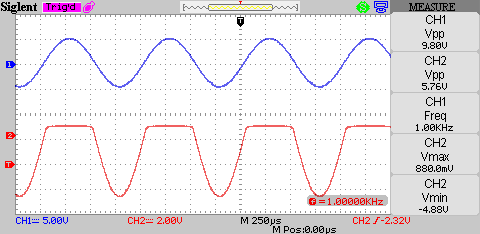
\includegraphics[scale=0.8]{./oscilloscope_captures/part4.png}
\end{center}
%
The waveforms captured using the oscilloscope show that the input waveform is clipped partially on the positive swing of the sine wave as expected. The oscilloscope measured the voltage ($V_{max}$) where the waveform is clipped to be approximately 880 mV. This clipped of region was zoomed in on the oscilloscope by increasing the volts per division, and the cursor mode was used to measure the cut off voltage more precisely (the oscilloscope has a 8 bit DAC, so the resolution is the displayed voltage range divided by 256). The cut off voltage was determined to be 700 mV. This value agrees with the prediction that the waveform will be clipped off at 0.7 volts because any voltages greater than 0.7 will cause the diode to conduct (holding a 0.7 volt drop across its terminals) and thus clip off the input signal at 0.7 volts. It also validates the voltage drop of a diode to be 700 mV.\par

\pagebreak

\subsection*{Part 5}
The objective of this part is to modify the circuit from \textit{Part 4} such that it will only pass negative input voltages. To do this, the voltage which the diode begins to conduct must be changed from 0.7 volts to zero volts relative to the output. An easy way to do this is to add a 0.7 volt source in series with the diode, such that the polarity of the source is opposite of the 0.7 volt drop across the diode. Conduction beginning at zero volts in this circuit causes positive voltages to be clipped off above 0 volts as the voltage drop remains essentially constant for any practical currents. All of the positive voltage in this case is dropped across resistor in accordance to Ohm's Law. This circuit is shown below:\par

\begin{center}
 \textbf{Figure 10.} Zero Volt Signal Clipper\\
 \begin{circuitikz}[american voltages]
   \draw
   (0,0)	to[sV, l=1 kHz 5V] (0,4)
    		to[R, l=500 $\Omega$, -*] (3,4)
    		to[Do] (3,2)
    		to[american voltage source, l_=0.7 V, -*] (3,0)
    		to (0,0)
   (3,4)	to[short, -o] (5,4)
   (3,0)	to[short, -o] (5,0)
   (5,4) to [open, v^=$v_{out}$]              (5,0);
 \end{circuitikz}
\end{center}
%
This circuit was constructed like shown in the diagram on a bread board, with the oscilloscope measuring the input on channel one and the output $V_{out}$ on channel two. Below in \textit{Figure 11} is a screen capture of the input and output waveforms of this circuit.\par
%
\vspace{12pt}\title{\textbf{Figure 11.} Oscilloscope Screen Capture.}
\begin{center}
 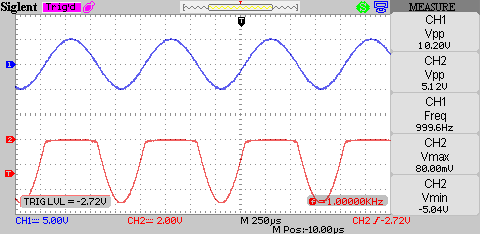
\includegraphics[scale=0.8]{./oscilloscope_captures/part5.png}
\end{center}

As expected the waveform is clipped off as the voltage the diode begins to conduct at is biased to 0V in this circuit, making the voltage measured by the oscilloscope zero for any positive input voltages. This validates the approach of biasing the voltage of the diode in the circuit to change the voltage which it conducts and clips.

\pagebreak

\subsection*{Part 6}
The objective of this part is similar to the last, except the circuit must be modified such that it will only pass voltages less than 2 volts. This can again be achieved by changing the voltage that the diode conducts from 0.7 volts to 2.0 volts relative to the output. This can be implemented by adding a 1.3 V voltage source in series with the diode (with the polarity in the same direction of the voltage drop on the resistor), causing the voltage drop across the two elements to be 2.0 volts when the diode conducts. For all voltages under two volts, the diode and supply will behave like an open circuit, allowing signals to freely pass. For input voltages above 2 volts the output will be held at the 2V drop. This circuit is shown in \textit{Figure 12}.\par
%
\begin{center}
 \textbf{Figure 12.} 2 Volt Signal Clipper\\
 \begin{circuitikz}[american voltages]
   \draw
   (0,0)	to[sV, l=1 kHz 5V] (0,4)
    		to[R, l=500 $\Omega$, -*] (3,4)
    		to[Do] (3,2)
   (3,0)	to[american voltage source, l=1.3 V, *-] (3,2)
   (3,0)	to (0,0)
   (3,4)	to[short, -o] (5,4)
   (3,0)	to[short, -o] (5,0)
   (5,4) to [open, v^=$v_{out}$]              (5,0);
 \end{circuitikz}
\end{center}
%
The circuit was assembled on a bread board and connected to the oscilloscope where channel 1 was connected to the input and channel to the output. The input and output waveforms and measurements were captured in \textit{Figure 13}.\par
%
\vspace{12pt}\title{\textbf{Figure 13.} Oscilloscope Screen Capture.}
\begin{center}
 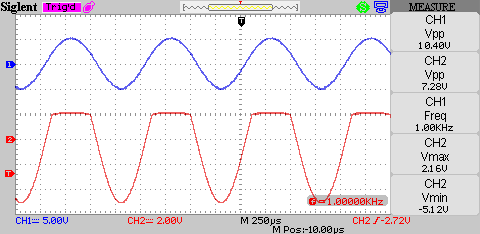
\includegraphics[scale=0.8]{./oscilloscope_captures/part6.png}
\end{center}
%
The waveform was clipped off above 2 volts like expected, confirming the predicted circuit and theory again.

\pagebreak

\subsection*{Part 7}
The circuit was again modified, this time such that an input signal would be cut off above 2 volts and below -2 volts. This circuit is implemented by adding another of the series diode and 1.3 volt supplies to the last circuit, this time with flipped polarity. This new circuit is shown below in \textit{Figure 14}. This circuit works because current will now flow through one of the sets of diodes and voltage supplies if the magnitude of the waveform exceeds 2 volts, causing the waveform to be clipped above above 2 volts and below -2 volts across the output. The excess voltage is again dropped across the resistor. \par
%
\begin{center}
 \textbf{Figure 14.} $\pm$ 2 Volt Clipper\\
 \begin{circuitikz}[american voltages]
   \draw
   (0,0)	to[sV, l=1 kHz 5V] (0,4)
    		to[R, l=500 $\Omega$, -*] (3,4)
    		to[Do] (3,2)
   (3,0)	to[american voltage source, l=1.3 V, *-] (3,2)
   (3,0)	to (0,0)
   (5,0)	to[Do, *-] (5,2)
   (5,4)	to[american voltage source, l=1.3V, *-] (5,2)
   (3,4)	to[short, -o] (7,4)
   (3,0)	to[short, -o] (7,0)
   (7,4) to [open, v^=$v_{out}$]              (7,0);
 \end{circuitikz}
\end{center}
%
The circuit was built by adding to the circuit from \textit{Part 6} a second diode and power supply connected in opposite polarity of the first. \textit{Figure 15} shows the oscilloscope capture of the input and output waveforms of this circuit.\par
%
\vspace{12pt}\title{\textbf{Figure 15.} Oscilloscope Screen Capture.}
\begin{center}
 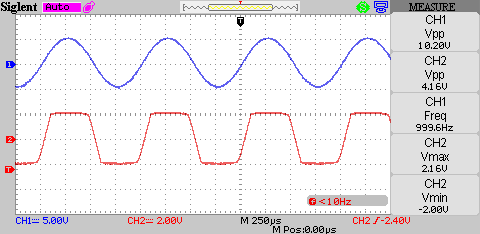
\includegraphics[scale=0.8]{./oscilloscope_captures/part7.png}
\end{center}
The output clips off at plus and minus 2 volts as expected.

\pagebreak

\subsection*{Part 8}
This final part is intended to show the response of the clipper circuit from \textit{Part 7} on square and triangle waves. It is expected that the circuit will have the same operation as before, clipping off each input waveform above 2 volts and below negative 2 volts. \textit{Figure 16} shows the circuit behavior for a square wave input and \textit{Figure 17} for a triangle wave.\par
%
\vspace{12pt}\title{\textbf{Figure 16.} Oscilloscope Screen Capture.}
\begin{center}
  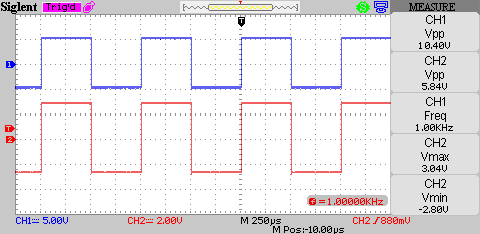
\includegraphics[scale=0.8]{./oscilloscope_captures/square.png}
\end{center}
%
\title{\textbf{Figure 17.} Oscilloscope Screen Capture.}
\begin{center}
  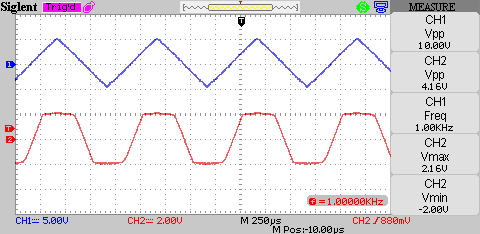
\includegraphics[scale=0.8]{./oscilloscope_captures/triangle.png}
\end{center}
%
For the square wave, the circuit doesn't behave as expected, cutting off at plus 3.04 volts and minus -2.80 volts instead of the expected plus and minus 2 volts. This appears to be a problem with the power supply being used, as the output voltages would not regulate down to the desired 1.3 volts, rather the lowest they would go to was about 2.1 volts. This problem is probably attributed to the fact that this circuit causes the PSU to sink current, which it likely is not intended to do nor can it properly regulate. The triangle wave did clip off as expected, cutting of at approximately plus and minus 2 volts. It is possible that the power supply only misbehaved on the square wave because the signal changes very rapidly on the rising and falling edges (compared to the other two waveforms), which may cause an error with the voltage control mechanism of the power supply.

%-----------------------------------------------------------------------------
%	Conclusion
%----------------------------------------------------------------------------------------
\section{Conclusion}

The I-V curve of an incandescent light bulb was found experimentally, showing that it is non-linear in nature. The I-V curve for the bulb was then used through load-line analysis to predict the current through the bulb with a resistor attached, which were verified to be correct experimentally. The behavior of a diode was then observed experimentally with an oscilloscope and was determined to behave as an open circuit until a voltage of approximately 0.7 volts is across its terminals from anode to cathode. After this voltage it was observed that the diode conducts and holds a nearly constant voltage drop of 0.7 volts. Understanding the constant voltage drop nature of the diode, several signal clipping circuits were designed to clip an input signal off at various voltage levels on the output of the circuit. This was done successfully by changing the voltage that the diode conducts (and accordingly the voltage drop) relative to the output, causing the waveform to be clipped at that voltage when it was exceeded and to pass signals below that voltage.

\end{document}